\chapter{Semantic Label Generation} \label{cha:labels}

The main objective of this work is concerned with predicting plausible layouts of retina structures and lesions.
We first approach this by using a GAN to generate semantic labels, trained on manual annotations.
By using a sophisticated generative model, we hope to be able to capture subtle relationships and interactions between the various different retinal structures, which would not be possible with classical data augmentation techniques.
Then we study how a heuristic-based method that samples from existing data in a ``naive'' way compares with the generative models.

In this section, we discuss the unique challenges of this task, and go on to compare three different approaches.

\section{Initial Experiments}

During the initial exploration phase for this task, we began by applying implementations of the most modern GAN designs, such as ContraGAN and StyleGAN.
To do this, we had to modify the generator and discriminator architectures to suit our problem domain, instead of creating RGB images.
Recall our semantic \emph{images} are represented as $M \in \mathbb{L}^{H \times W}$, where $\mathbb{L} = \{0, ..., 9\}$.
To extract the one-hot encoded (w.r.t each pixel) semantic \emph{label} representation, we extract the appropriate labels from this image, to get the desired input $S \in \{ 0, 1 \}^{C \times H \times W}$.
The final layer of the generator becomes a softmax layer, which allows us to interpret each pixel of the output feature map $P \in \mathbb{R}^{C \times H\times W}$ as the probability of that pixel belonging to each class; that is:
\begin{align}
    \forall h \in H, \ \forall w \in W \quad \sum_{c}^C P_{chw} = 1 \text{ and } P_{chw} \geq 0
\end{align}
To recover the semantic image representation, we simply take the arg max of this probability map over the channels.
\begin{align}
    M = \argmax_c P    
\end{align}
This relationship between these representations is depicted graphically in \Cref{fig:semantic_label}.

\begin{figure}[h]
    \centering
    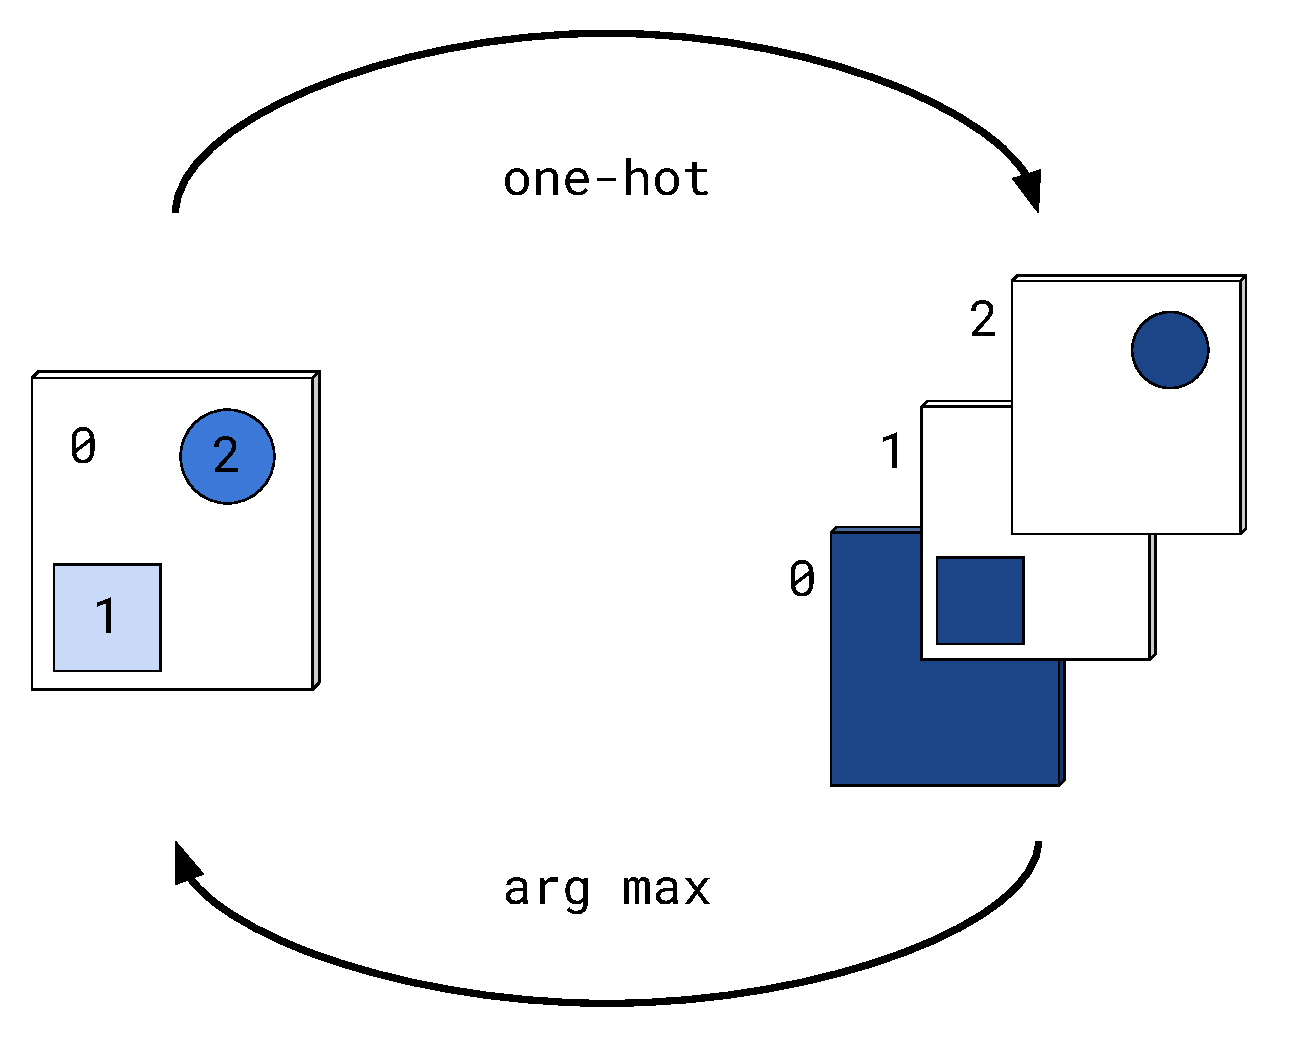
\includegraphics[width=0.5\textwidth]{labels/figs/label-semantics.pdf}
    \caption{Converting between the integer-encoded semantic image and one-hot encoded semantic label representation.}
    \label{fig:semantic_label}
\end{figure}

However, we quickly discovered that these architectures -- primarily concerned with creating high-fidelity, dense, natural, 3-channel images -- collapsed almost immediately, before generating any useful outputs.
In particular, we found that GAN architectures which utilised a ResNet-based discriminator were particularly problematic, even when the capacity of the generator, in terms of the number of parameters, was much greater.
Interestingly, this was not reported by any of the (admittedly limited) existing literature, which largely use architectures based on conventional CNNs.

We theorise that this is because the sparse nature of the semantic labels, coupled with the large number of channels, made it a challenge for the generator to create plausible outputs, while the discriminator learnt very quickly to distinguish real and fake images.
Hence, it was established that we would need to create a bespoke architecture starting from first principles, based on an understanding of what made the task challenging, and how these issues could be mitigated.

\section{ACGAN}

\begin{figure}
    \centering
    \begin{subfigure}{\textwidth}
        \centering
        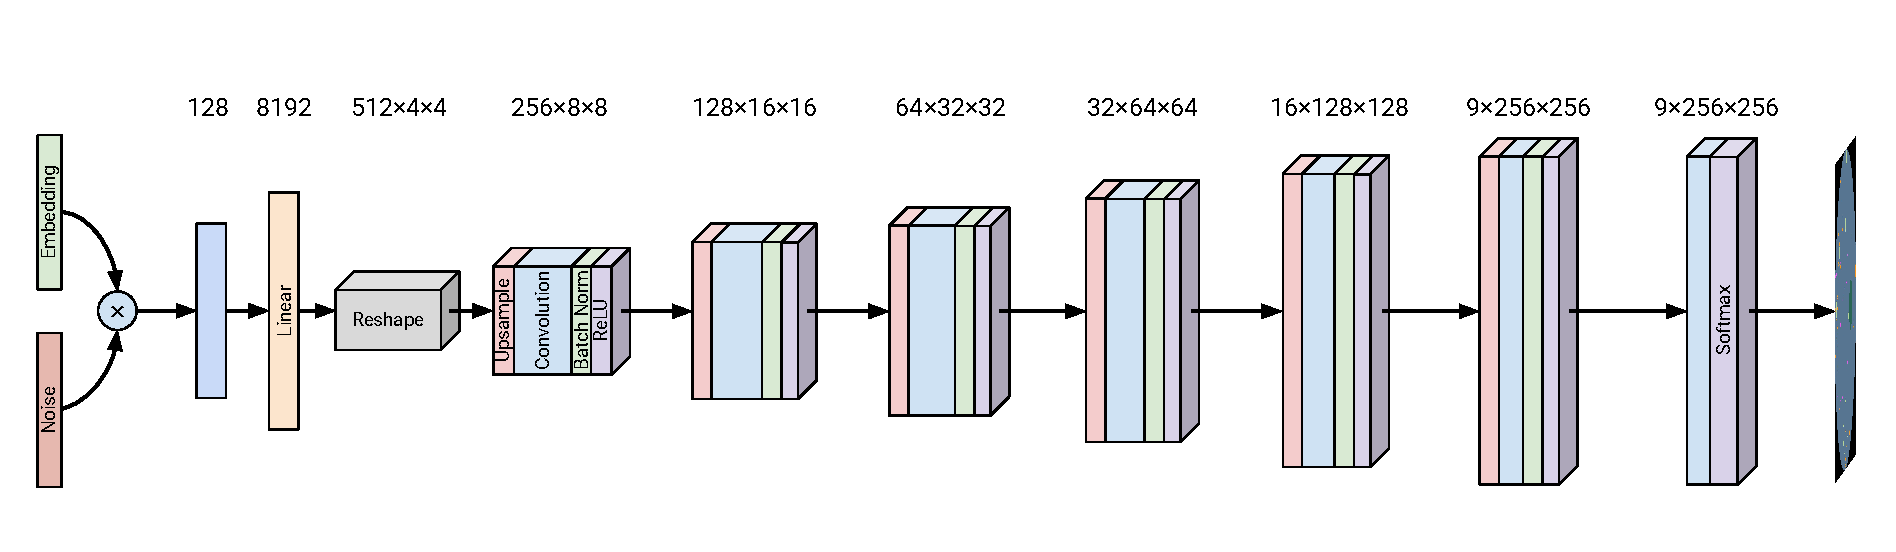
\includegraphics[width=\linewidth]{labels/figs/acgan-generator.pdf}
        \caption{ACGAN generator architecture.}
        \label{fig:acgan_gen}
    \end{subfigure}
    \begin{subfigure}{\textwidth}
        \centering
        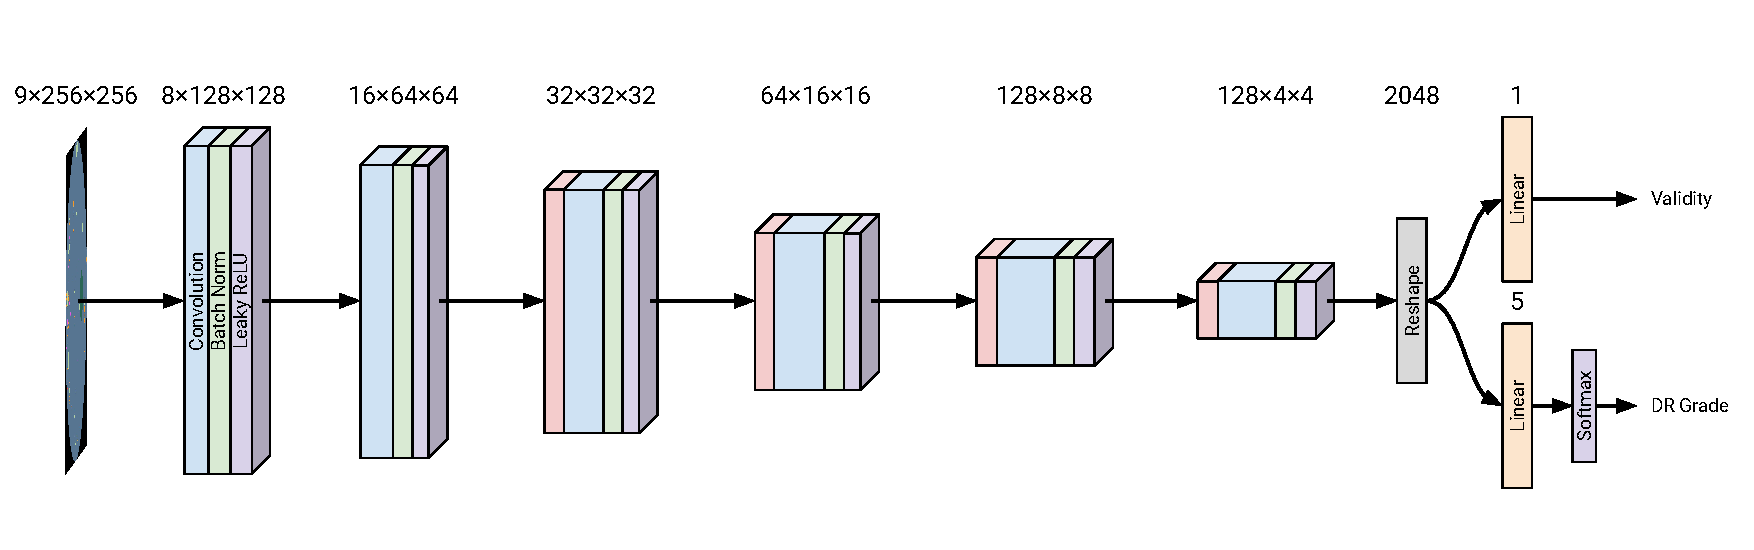
\includegraphics[width=\linewidth]{labels/figs/acgan-discriminator.pdf}
        \caption{ACGAN discriminator architecture.}
        \label{fig:acgan_dis}
    \end{subfigure}
    \caption{ACGAN network architectures.}
    \label{fig:acgan_arch}
\end{figure}

Motivated by this, we designed a DCGAN-based generator and discriminator architecture to generate class-conditioned semantic labels, using auxiliary discriminator losses (ACGAN).
In this conditioning strategy, we add a classification layer to the end of the discriminator which learns to predict the class of the input image \cite{odena2017conditional}.
As the generator attempts to minimise this auxiliary loss, the quality of conditioning will increase.

The generator creates images at a resolution of $256 \times 256$;  we found that attempting to use this architecture to generate images at higher resolutions than this greatly increased instability, since discriminability increases with resolution.
To condition the generator, we take the Hadamard product between the latent noise vector $z$ and the embedded representation of the image class.
Generated images are upsampled to $512 \times 512$ using bilinear interpolation (and then thresholded to valid values) as a post-processing step.

Where this design departs from conventional ACGANs, as presented in their original form, is the asymmetry between the generator capacity (2,672,630 parameters) and discriminator capacity (259,070 parameters).
Limiting the discriminator in terms of both the number of parameters and other training techniques, detailed in the following sections, were key in allowing for stable training.

\subsection{Optimiser}

We use the Adam optimiser with $\alpha_G = 0.0005$ and $\alpha_D = 0.0001$ with $\beta_1=0.5$, $\beta_2=0.999$.
Two generator training iterations are performed for each discriminator training iteration.
This imbalanced learning allowed the generator to keep up with the discriminator, and was critical to prevent training from collapsing.

\subsection{One-Sided Label Smoothing}

Label smoothing is a technique where the target values of 1 and 0 are replaced by ``smoothed'' labels such as $\alpha=0.9$ for the positive value and $\beta=0.1$ for the negative value.
This yields the new optimal discriminator 
\begin{align}
    D(x) = \frac{\alpha p_{data}(x) + \beta p_{model}(x)}{p_{data}(x) + p_{model}(x)}
\end{align}
However, when $\beta \neq 0$, $p_{data} \approx 0$, and $p_{model}$ is large, erroneous samples from $p_{model}$ have no incentive to move nearer to the data.
Hence, we smooth only the positive labels to $\alpha = 0.9$, and leave the negative examples as 0 \cite{salimans2016}.
This has the effect of penalising the discriminator for being overconfident.

\subsection{Loss Functions} \label{sec:hingeloss}

For the discriminator, we use the Hinge loss \cite{lim2017geometric}.
Inspired by its use in SVMs, it aims to find a separating hyperplane between real and fake samples. 
The generator attempts to decrease the margin, whereas the discriminator attempts to increase it.
This allows for strong gradients, even with a confident discriminator.
\begin{align}
    \mathcal{L}^D_{adv} &= -\mathbb{E}_x [\min(0, -1+D(x)] - \mathbb{E}_z [\min(0, -1-D(G(z)))]
\end{align}
To implement the ACGAN, we also use auxiliary losses.
\begin{align}
    \mathcal{L}^D_{aux} = \mathbb{E}[\log P(y | x)] + \mathbb{E}[\log P(y | G(z|y)]
\end{align}
For the generator, we use the comparatively simple Wasserstein loss.
\begin{align}
    \mathcal{L}^G &= -\mathbb{E}_z[D(G(z))]
\end{align}

\subsection{Adaptive Discriminator Augmentation}

Adaptive Discriminator Augmentation (ADA) \cite{karras2020training} is a technique developed to prevent the discriminator from overfitting when training a GAN on limited data.
Various transformations are applied to all images seen by the discriminator (real and fake) with probability $p$, where $p$ is determined by the degree of overfitting exhibited by the discriminator.
A simple heuristic is used to determine how much the discriminator is overfitting:
\begin{align}
    r_t = \mathbb{E}[\text{sign}(D_{train})]
\end{align}
On each training iteration, $p$ is incremented or decremented by a fixed value depending on the value of $r_t$.

We found that ADA was crucial to prevent discriminator overfitting. 
Typically, GANs are trained with many thousands of images, which provides enough diversity to prevent overconfidence in the discriminator.
However, since our training set is small, it is easy for the discriminator to overfit relatively early on in training.
The transforms we use are probabilistic rotations, affine transforms, and Gaussian noise.

For the rotation, we apply a 90 degree rotation up to 4 times, as detailed in the original paper.
When rotating, the background is filled by setting the background channel to 1 and all other channels to 0.

\begin{lstlisting}[language=Python, caption=Python-like pseudocode for probabilistic rotation.]
def probabilistic_rotate(x: Tensor, p: float) -> Tensor:
    """
    Rotates a tensor x of shape (C, H, W) with probability p.
    """
    if random() > p:
        return x
        
    # Randomly choose a number of rotations.
    num_rotations = random_choice([0, 1, 2, 3, 4])
    
    fill = get_fill_colour(x)
    
    # Rotate by multiples of 90 degrees.
    x = rotate(x, 90 * num_rotations, fill=fill)
    return x
    
def get_fill_colour(x: Tensor) -> List:
    # Only fill the background to 1s.
    n_channels, _, _ = x.shape
    fill = [1] + [0 for _ in range(n_channels - 1)]
    return fill 
\end{lstlisting}
For the affine transformation, we perform a random scale, translation, and (fine-grained) rotation.
By ``random'', we mean that the parameters of the transformation itself are also sampled randomly from the specified ranges, in addition to the probability $p$ of the ADA transformation being applied in the first place.
\begin{lstlisting}[language=Python, caption=Python-like pseudocode for probabilistic affine rotation.]
def probabilistic_affine(x: Tensor, p: float) -> Tensor:
    """
    Performs a random affine transformation on tensor x of shape (C, H, W) with probability p.
    """
    if random() > p:
        return x
        
    fill = get_fill_colour(x)

    x = random_translate(x, (0.5, 0.5), fill=fill)
    x = random_scale(x, (0.8, 1.2), fill=fill)
    x = random_rotate(x, 360, fill=fill)
    return x
\end{lstlisting}
For the Gaussian noise, we also scale the standard deviation of the noise with the degree of overfitting, up to a specified maximum.
\begin{lstlisting}[language=Python, caption=Python-like pseudocode for probabilistic Gaussian noise.]
MEAN = 0
MAX_STD = 1.0

def probabilistic_noise(x: Tensor, p: float, mean: float, max_std: float) -> Tensor:
    """
    Adds noise to a tensor x of shape (C, H, W) with probability p.
    """
    if random() > p:
        return x

    # Scale the standard deviation of the noise based on the probability
    # i.e. degree of overfitting.
    std = p * MAX_STD
    noise = MEAN + normal_distribution(x.shape) * std
    return x + noise
\end{lstlisting}

We set 0.6 as the target value for $r_t$, and $p$ is capped at a maximum of 0.85, as the authors suggest that past this point the transforms will start to ``leak'' -- meaning that they will begin to occur in the generated images.
The value of $p$ is adjusted by by 0.01 on each batch iteration.

%\begin{lstlisting}[language=Python]
%TARGET_ADA_R = 0.6
%MAX_P = 0.85
%
%def ada_transform(images: Tensor, p: float) -> Tensor:
%    transforms = [
%        probabilistic_rotate,
%        probabilistic_affine,
%        probabilistic_noise,
%    ]
%    for i in range(batch_size):
%        img = images[i]
%        for t in transforms:
%            img = t(img, p)
%            
%    return images
%
%def train(generator: Generator, discriminator: Discriminator):
%    ada_r = 0.0
%    for real_images, fake_images in data:
%        transformed_real_images = ada_transform(real_imgs)
%        real_pred = discriminator(transformed_real_images)
%        
%        ada_r = mean(sign(real_pred))
%        ...    
%        fake_images = generator(noise)
%        transformed_fake_images = ada_transform(fake_images)
%        fake_pred = discriminator(transformed_fake_images)
%        
%        discriminator_loss = compute_loss(real_pred, fake_pred)
%        ...
%        if ada_r > TARGET_ADA_R:
%            p += 0.01
%        if ada_r < TARGET_ADA_R:
%            p -= 0.01
%        
%        p = max(0, p)
%        p = min(p, MAX_P)
%\end{lstlisting}

\subsection{Weight Initialisation}

Weights are initialised using a normal distribution $\mathcal{N}(0, 0.02)$.
We also experimented with orthogonal initialisation, but found it was more prone to collapse.

\section{ProGAN}

% DataParallel(
%   (module): Discriminator(
%     (layers): ModuleList(
%       (0): DisGeneralConvBlock(
%         (conv_1): EqualizedConv2d(64, 64, kernel_size=(3, 3), stride=(1, 1), padding=(1, 1))
%         (conv_2): EqualizedConv2d(64, 128, kernel_size=(3, 3), stride=(1, 1), padding=(1, 1))
%         (downSampler): AvgPool2d(kernel_size=2, stride=2, padding=0)
%         (lrelu): LeakyReLU(negative_slope=0.2)
%       )
%       (1): DisGeneralConvBlock(
%         (conv_1): EqualizedConv2d(128, 128, kernel_size=(3, 3), stride=(1, 1), padding=(1, 1))
%         (conv_2): EqualizedConv2d(128, 256, kernel_size=(3, 3), stride=(1, 1), padding=(1, 1))
%         (downSampler): AvgPool2d(kernel_size=2, stride=2, padding=0)
%         (lrelu): LeakyReLU(negative_slope=0.2)
%       )
%       (2): DisGeneralConvBlock(
%         (conv_1): EqualizedConv2d(256, 256, kernel_size=(3, 3), stride=(1, 1), padding=(1, 1))
%         (conv_2): EqualizedConv2d(256, 512, kernel_size=(3, 3), stride=(1, 1), padding=(1, 1))
%         (downSampler): AvgPool2d(kernel_size=2, stride=2, padding=0)
%         (lrelu): LeakyReLU(negative_slope=0.2)
%       )
%       (3): DisGeneralConvBlock(
%         (conv_1): EqualizedConv2d(512, 512, kernel_size=(3, 3), stride=(1, 1), padding=(1, 1))
%         (conv_2): EqualizedConv2d(512, 512, kernel_size=(3, 3), stride=(1, 1), padding=(1, 1))
%         (downSampler): AvgPool2d(kernel_size=2, stride=2, padding=0)
%         (lrelu): LeakyReLU(negative_slope=0.2)
%       )
%       (4): DisGeneralConvBlock(
%         (conv_1): EqualizedConv2d(512, 512, kernel_size=(3, 3), stride=(1, 1), padding=(1, 1))
%         (conv_2): EqualizedConv2d(512, 512, kernel_size=(3, 3), stride=(1, 1), padding=(1, 1))
%         (downSampler): AvgPool2d(kernel_size=2, stride=2, padding=0)
%         (lrelu): LeakyReLU(negative_slope=0.2)
%       )
%       (5): DisGeneralConvBlock(
%         (conv_1): EqualizedConv2d(512, 512, kernel_size=(3, 3), stride=(1, 1), padding=(1, 1))
%         (conv_2): EqualizedConv2d(512, 512, kernel_size=(3, 3), stride=(1, 1), padding=(1, 1))
%         (downSampler): AvgPool2d(kernel_size=2, stride=2, padding=0)
%         (lrelu): LeakyReLU(negative_slope=0.2)
%       )
%       (6): DisGeneralConvBlock(
%         (conv_1): EqualizedConv2d(512, 512, kernel_size=(3, 3), stride=(1, 1), padding=(1, 1))
%         (conv_2): EqualizedConv2d(512, 512, kernel_size=(3, 3), stride=(1, 1), padding=(1, 1))
%         (downSampler): AvgPool2d(kernel_size=2, stride=2, padding=0)
%         (lrelu): LeakyReLU(negative_slope=0.2)
%       )
%       (7): ConDisFinalBlock(
%         (conv_1): EqualizedConv2d(513, 512, kernel_size=(3, 3), stride=(1, 1), padding=(1, 1))
%         (conv_2): EqualizedConv2d(512, 128, kernel_size=(4, 4), stride=(1, 1))
%         (conv_3): EqualizedConv2d(128, 1, kernel_size=(1, 1), stride=(1, 1))
%         (label_embedder): Embedding(5, 128)
%         (batch_discriminator): MinibatchStdDev(group_size=4)
%         (lrelu): LeakyReLU(negative_slope=0.2)
%       )
%     )
%     (from_rgb): ModuleList(
%       (0): Sequential(
%         (0): EqualizedConv2d(9, 64, kernel_size=(1, 1), stride=(1, 1))
%         (1): LeakyReLU(negative_slope=0.2)
%       )
%       (1): Sequential(
%         (0): EqualizedConv2d(9, 128, kernel_size=(1, 1), stride=(1, 1))
%         (1): LeakyReLU(negative_slope=0.2)
%       )
%       (2): Sequential(
%         (0): EqualizedConv2d(9, 256, kernel_size=(1, 1), stride=(1, 1))
%         (1): LeakyReLU(negative_slope=0.2)
%       )
%       (3): Sequential(
%         (0): EqualizedConv2d(9, 512, kernel_size=(1, 1), stride=(1, 1))
%         (1): LeakyReLU(negative_slope=0.2)
%       )
%       (4): Sequential(
%         (0): EqualizedConv2d(9, 512, kernel_size=(1, 1), stride=(1, 1))
%         (1): LeakyReLU(negative_slope=0.2)
%       )
%       (5): Sequential(
%         (0): EqualizedConv2d(9, 512, kernel_size=(1, 1), stride=(1, 1))
%         (1): LeakyReLU(negative_slope=0.2)
%       )
%       (6): Sequential(
%         (0): EqualizedConv2d(9, 512, kernel_size=(1, 1), stride=(1, 1))
%         (1): LeakyReLU(negative_slope=0.2)
%       )
%       (7): Sequential(
%         (0): EqualizedConv2d(9, 512, kernel_size=(1, 1), stride=(1, 1))
%         (1): LeakyReLU(negative_slope=0.2)
%       )
%     )
%   )
% )


\begin{figure}[h]
    \centering
    \begin{subfigure}{\textwidth}
        \centering
        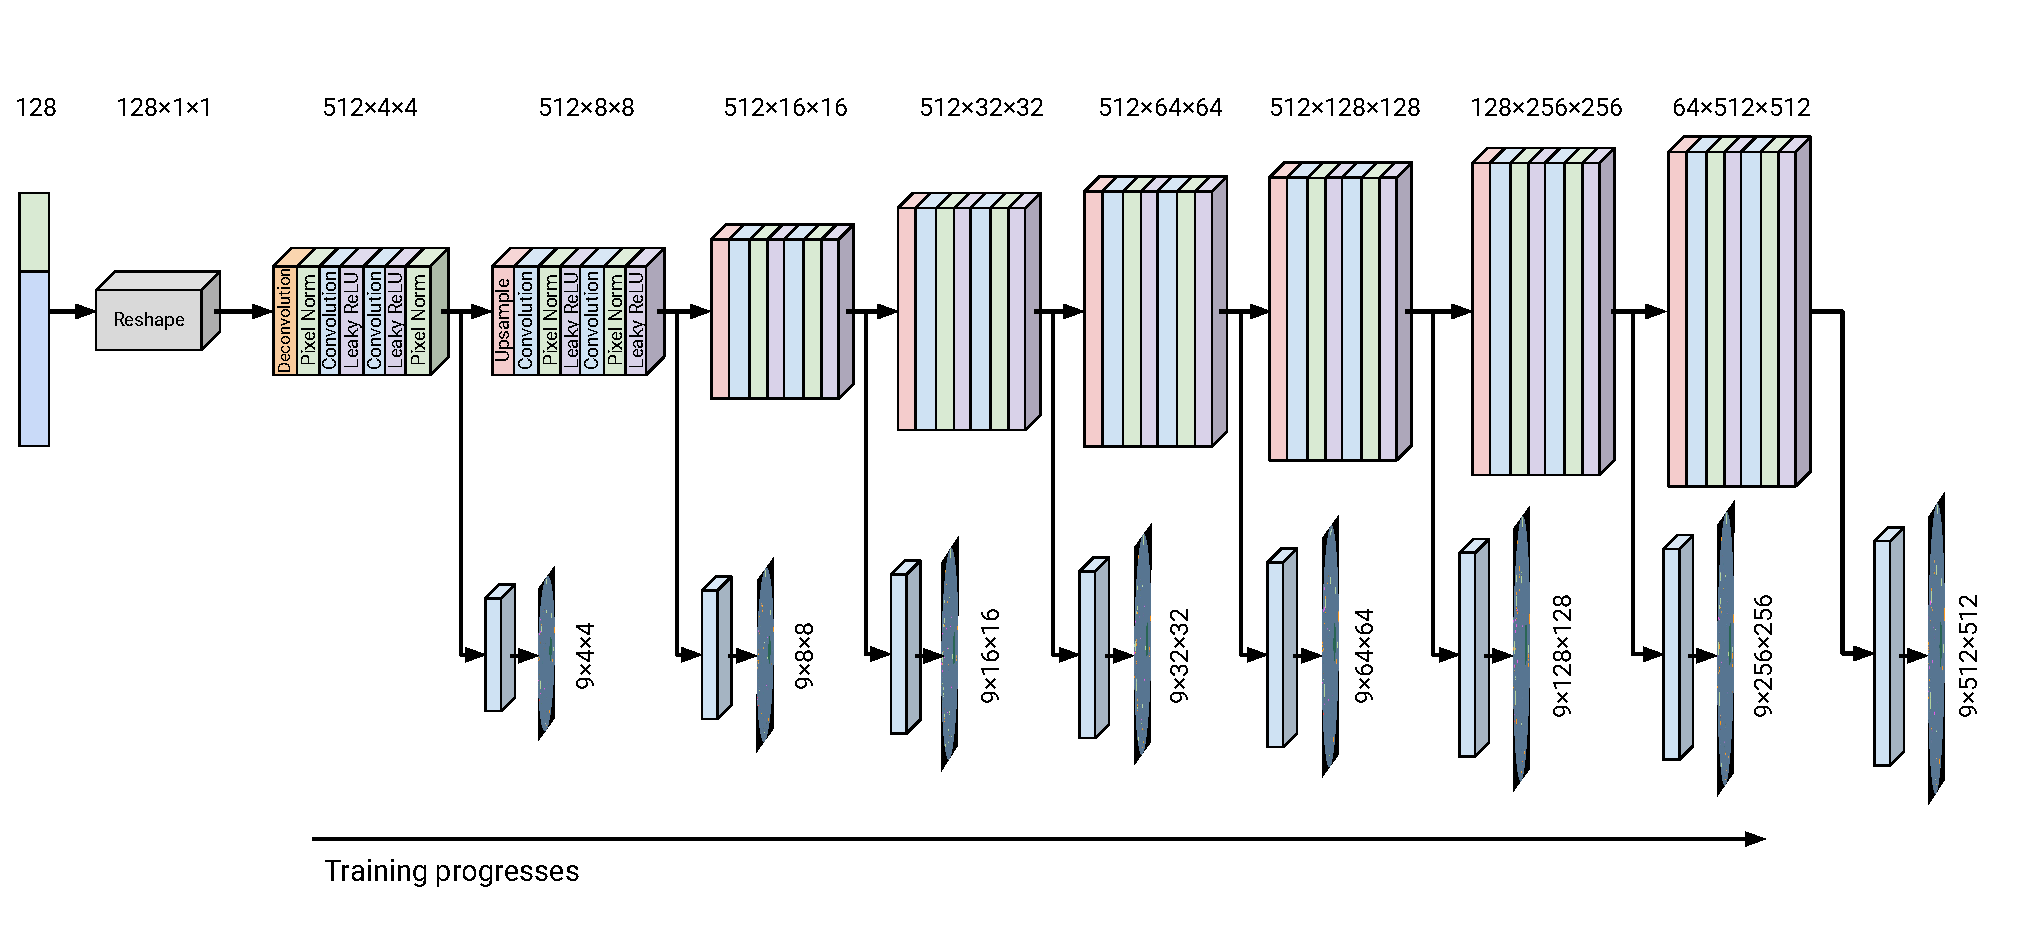
\includegraphics[width=\linewidth]{labels/figs/progan-generator.pdf}
        \caption{ProGAN generator architecture.}
        \label{fig:progan_gen}
    \end{subfigure}
    \begin{subfigure}{\textwidth}
        \centering
        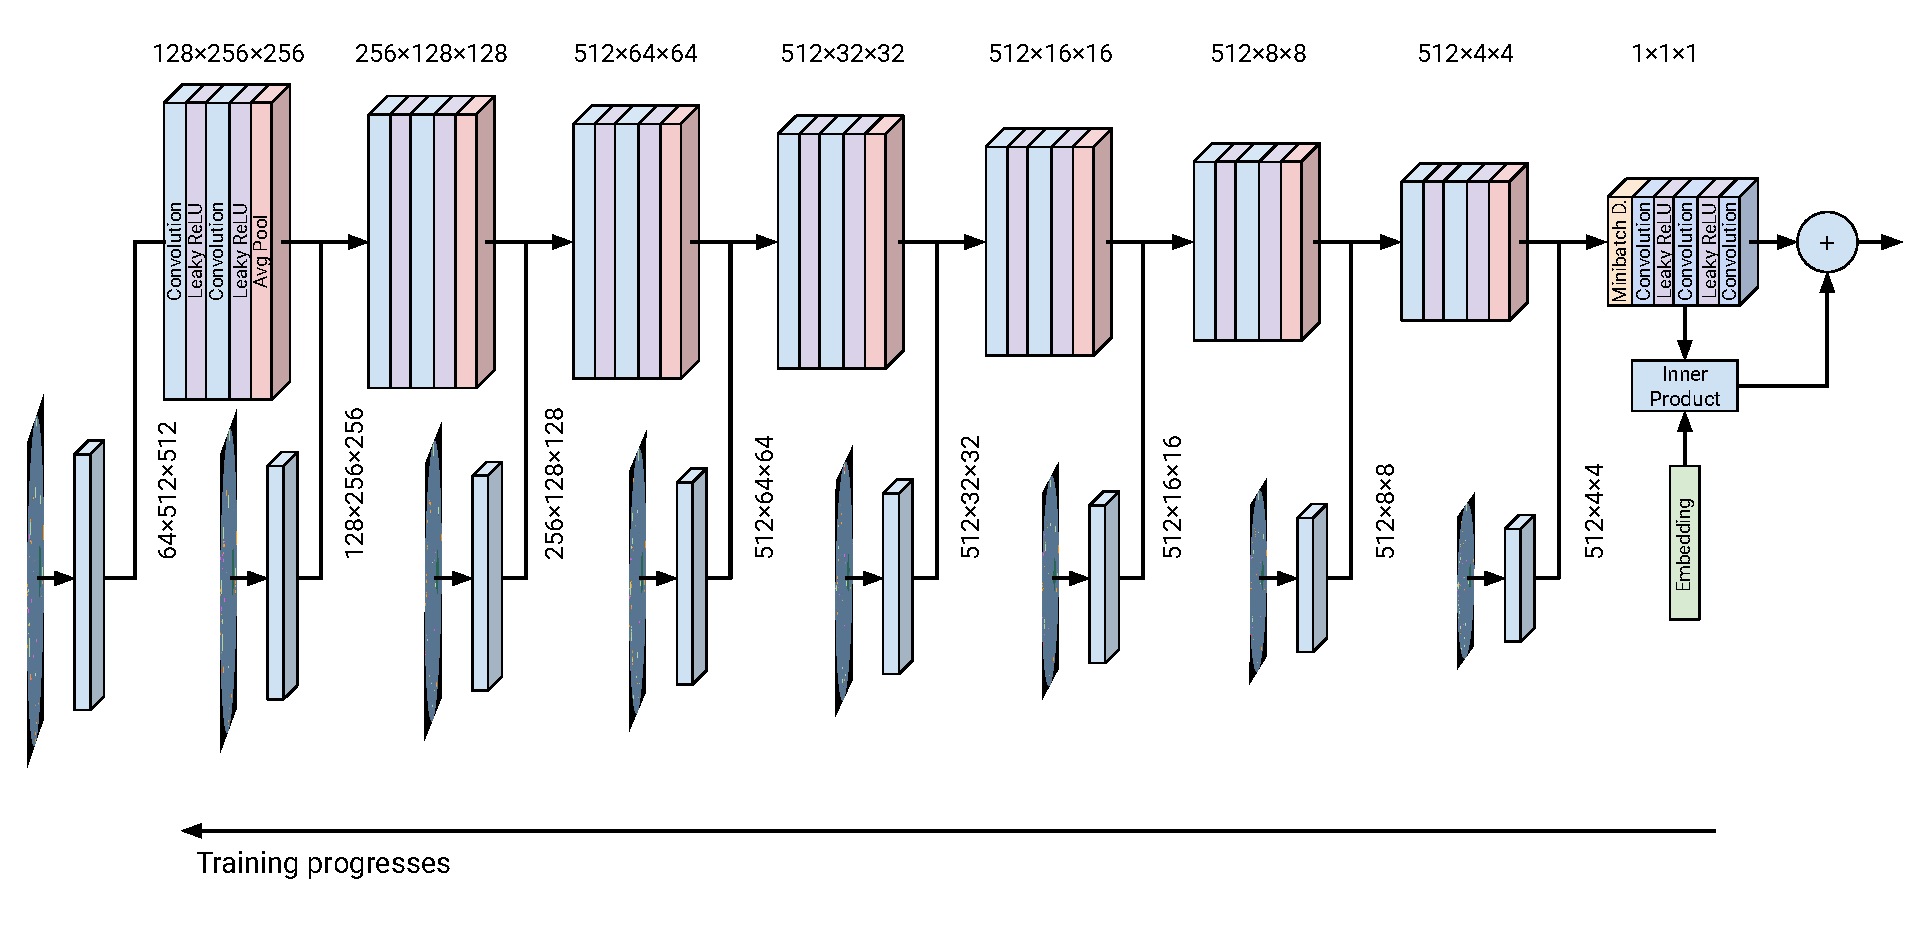
\includegraphics[width=\linewidth]{labels/figs/progan-discriminator.pdf}
        \caption{ProGAN discriminator architecture.}
        \label{fig:progan_dis}
    \end{subfigure}
    \caption{ProGAN network architectures.}
    \label{fig:progan_arch}
\end{figure}

As discussed, much of the instability we experienced when attempting to train semantic label generation GANs was owing to the discriminator's confidence, and the generator being unable to ``catch up''.
We also know that higher resolution images are more discriminable than lower resolution images.
Hence, it's intuitive that by starting at lower resolutions and progressively growing the generator and discriminator -- and therefore the resolution at which they operate -- the networks will be appropriately balanced throughout training.
Indeed, we found this to be the case, and that by allowing the generator to start with very small resolutions, the use of a ResNet-based discriminator was possible.
The generator and discriminator capacities are also very balanced, particularly in comparison to the ACGAN, with the generator having 24,639,137 parameters and the discriminator 24,646,209.


We use a ProGAN architecture to generate images starting from a resolution of $4\times 4$ up to $512\times 512$.
The generator and discriminator architectures are depicted in \Cref{fig:progan_arch}, with each additional block being capable of generating or discriminating images at a greater resolution.
In order to support variable sized images during training, we use \lstinline{toRGB} blocks in the generator, which are simply $1\times 1$ convolutions that reduce the number of feature maps down to the nine required in the output.
This allows us to create images at different resolutions while retaining the parameters learned in the prior hidden layers.
Conversely, \lstinline{fromRGB} blocks are used in the discriminator to increase the number of feature maps. 

We retain many of the same techniques detailed above, including label smoothing, the same loss function, and ADA.
However, we found that techniques that we relied upon with the fixed-resolution ACGAN, such as ADA, had a significantly weaker effect here.
We also incorporate some of the improvements detailed in the original ProGAN paper such as equalised learning rates and pixelwise feature vector normalisation in the generator \cite{DBLP:journals/corr/abs-1710-10196}.

To condition the generator, we simply concatenate the one-hot encoding of the class with the latent noise vector $z$.
We also experimented with using categorical batch normalisation as the conditioning strategy, but found that this caused mode collapse within each class.

\subsection{Optimiser}

We use the Adam optimiser with $\alpha_G = 0.0005$, $\alpha_D= 0.0001$, $\beta_1 = 0.0$, $\beta_2 = 0.99$ (same $\beta$ values as in the original ProGAN paper).
Unlike the ACGAN configuration, we perform just one generator training iteration for each discriminator training iteration.

\subsection{Equalised Learning Rate}

We use an equalised learning rate, where weights are initialised in the first instance using $\mathcal{N}(0, 1)$, and scaled dynamically during training.
Specifically, we set
\begin{align}
    \hat{w_i} = \frac{w_i}{c}
\end{align}
where $c$ is the per-layer normalisation constant from He initialisation \cite{he2015delving},
\begin{align}
    c = \sqrt{\frac{2}{n_l}}
\end{align}
and $n_l$ is the number of neurons in a layer.

\subsection{Pixelwise Feature Vector Normalisation}

We scale the feature vector of each pixel to unit length after each convolutional layer to prevent excessive signal magnitudes.
For the feature vector at pixel $(x, y)$, $a_{x, y}$, we obtain the normalised feature vector $b_{x, y}$ by
\begin{align}
        b_{x, y} = \frac{a_{x, y}}{\sqrt{\frac{1}{N} \sum_{j=0}^{N-1} a^i_{x, y} + \epsilon}}
\end{align}
where $N$ is the number of feature maps and $\epsilon = 10^{-8}$.

\subsection{Minibatch Standard Deviation}

In this technique, we first compute the standard deviation over each feature and spatial location in a minibatch.
We take the average of these standard deviations to yield a single value, which is then repeated and appended as an additional feature map.

\subsection{Projection Discriminator}

Introduced by \citeauthor{miyato2018cgans} \cite{miyato2018cgans}, in a projection discriminator, a projection between the feature maps and condition is added to the discriminator output.
This is computed as
\begin{align}
    f(x, y) = y^\intercal V \phi(x) + \psi (\phi(x))
\end{align}
where $x$ is the feature vector, $y$ is the class, and $V$ is the class embedding matrix -- making $y^\intercal V$ the corresponding embedding vector.
The transformations $\phi$ and $\psi$ are implemented as convolutional layers. 

\subsection{Training}

For each fade-in phase, we calculate the alpha value to merge images from the new and old resolution.
We spend 50\% of each phase fading in the previous resolution using a residual block to ``merge'' the new and old resolutions.
The length of each phase in the training regime is shown in \Cref{tab:progan_training}.

\begin{table}[h]
    \centering
    \begin{tabular}{lccccccccc}
        \toprule
        Resolution & $4^2$ & $8^2$ & $16^2$ & $32^2$ & $64^2$& $128^2$& $256^2$& $512^2$ \\
        \midrule
        Epochs & 20 & 40 & 60 & 80 & 100 & 120 & 140 & 160 \\
        Batch size & 512 & 256 & 128 & 64 & 32 & 16 & 8 & 4 \\
        \bottomrule
    \end{tabular}
    \caption{ProGAN training phases.}
    \label{tab:progan_training}
\end{table}

% \begin{figure}[h]
%     \centering
%     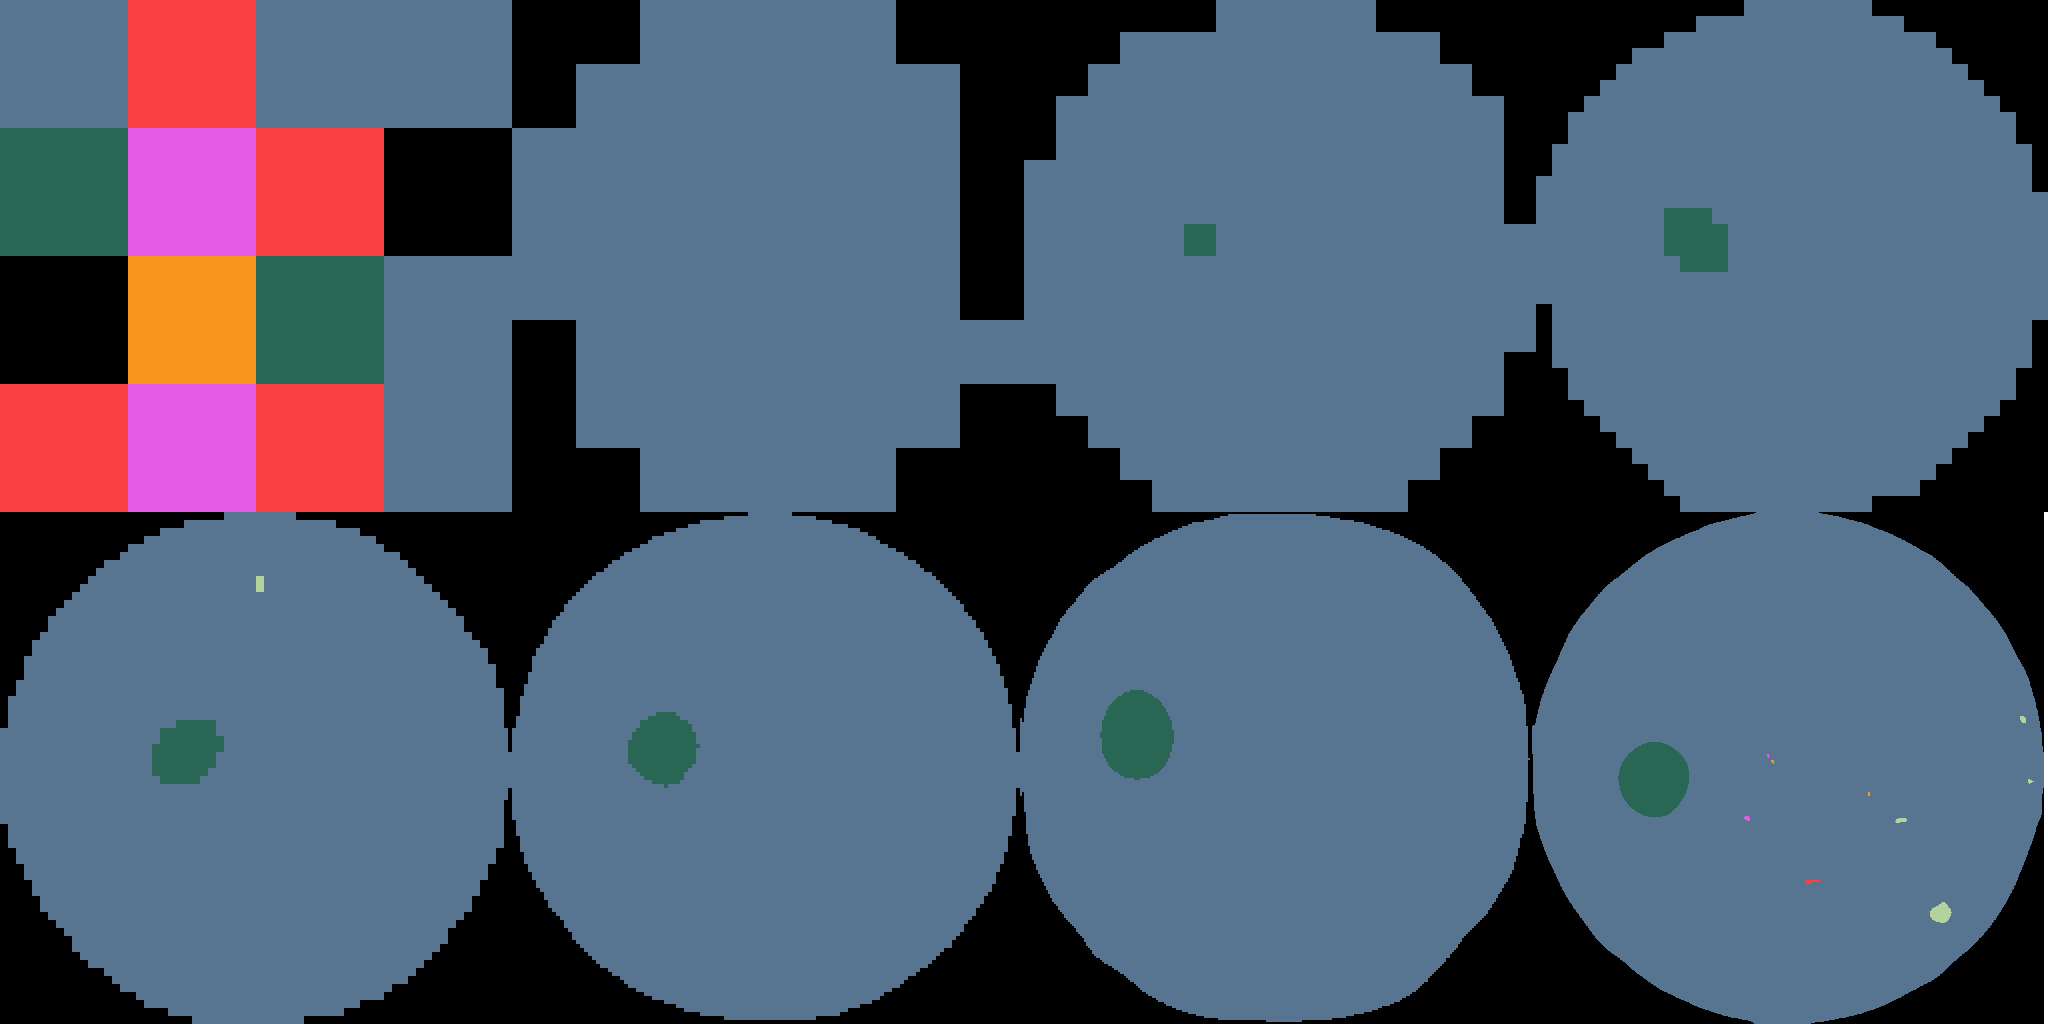
\includegraphics[width=0.5\textwidth]{labels/figs/progressive-growing.png}
%     \caption{Samples taken during training at resolutions from $4\times 4$ to $512 \times 512$.}
%     \label{fig:progressive_grow}
% \end{figure}
% 
%  as shown in \Cref{fig:progressive_grow}.

\section{Copy-Paste}

\begin{figure}[h]
    \centering
    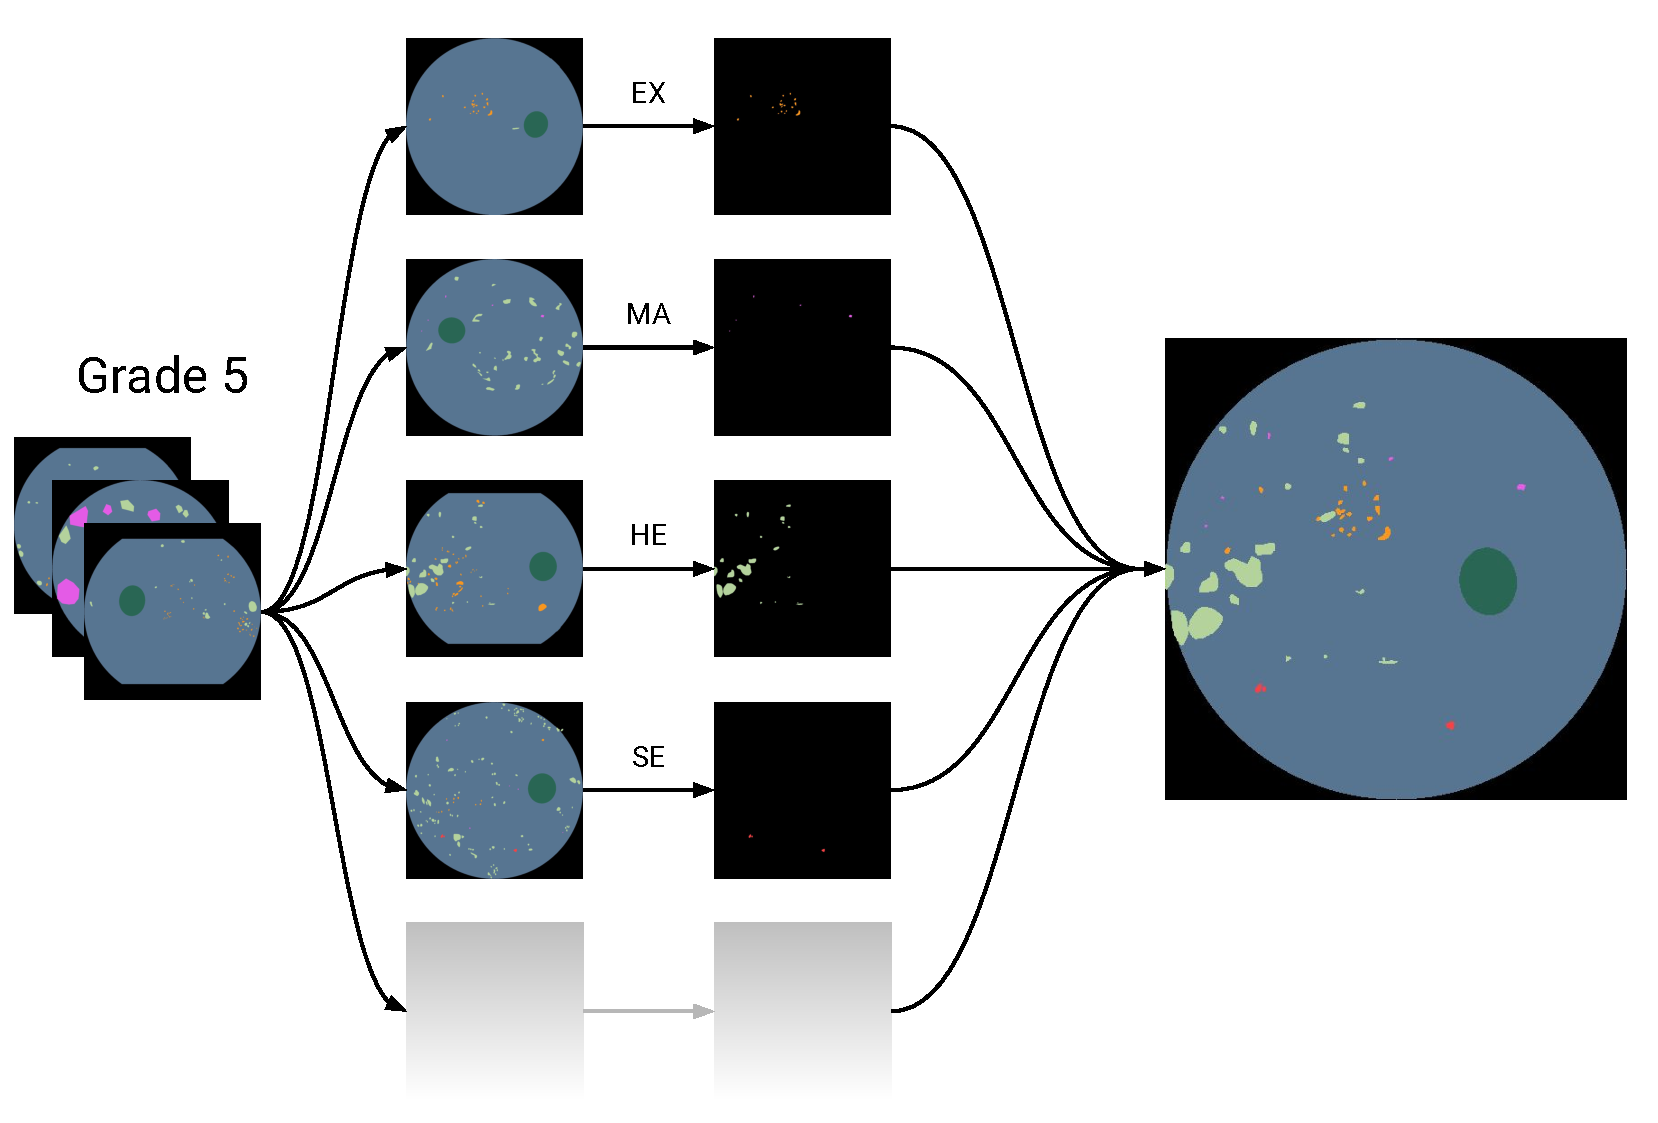
\includegraphics[width=0.6\textwidth]{labels/figs/copy-paste}
    \caption{Illustration of copy-paste generation.}
    \label{fig:copypaste}
\end{figure}

\citeauthor{ghiasi2020simple} \cite{ghiasi2020simple} showed that simply copy-and-pasting objects onto a scene can improve the performance of instance segmentation algorithms on natural images.
Inspired by this, we introduce a simple and efficient data augmentation technique that uses multi-label sampling to generate new data for semantic segmentation.
We refer to this technique as ``copy-paste''.
To generate copy-pasted data, semantics labels for each class are randomly sampled from existing data and concatenated in order to create a new semantic label of the same grade.
This process is depicted in \Cref{fig:copypaste}.

The advantages of this method are clear in that it requires very few compute resources and no prior training, while still being able to create a diverse range of samples.
It is only possible because the layout of each image is uniform, and we are not limited by rigid structures such as vessels (which are filled in by the image-to-image translation network).
In this sense, retinal fundus images are a very flexible target modality -- the same method would be difficult to apply on, for example, the Cityscapes dataset.

Of course, this approach does not take into account any knowledge \emph{a posteriori} about the retinal structure or relationship between lesions.
Hence, images generated using this method can exhibit overlapping, or implausible semantic labels.
Nevertheless, these same issues can arise with GANs; it may even be the case that certain lesions are simply too difficult or too small for the GANs (in their current form) to generate, whereas copy-paste has no such limitations.

As before, we take care to prevent data leakage by sampling new data points from only the fixed training set.
We could also apply scale and position jittering to further increase diversity, but we leave this as a future investigation.

\section{Experiments}

For all ACGAN experiments, we set the batch size to 64 and trained for 2000 epochs.
Early experiments included ``slow'' (e.g. 100 generator, 100 discriminator iterations per batch) and ``fast'' (e.g. 1 generator, 1 discriminator iteration per batch) training schemes, and exploring different variants on ADA, such as annealing the maximum $p$ value over time, or tweaking the types of transformation.
Rather predictably, any change that increased the probability of discriminator overfitting was likely to cause training to collapse.
We also test a variant of the ACGAN where we condition the generator by concatenating the embedded class vector with the latent dimension, instead of taking the Hadamard product.

\begin{figure}[h]
    \centering
    \begin{subfigure}{0.45\textwidth}
        \centering
        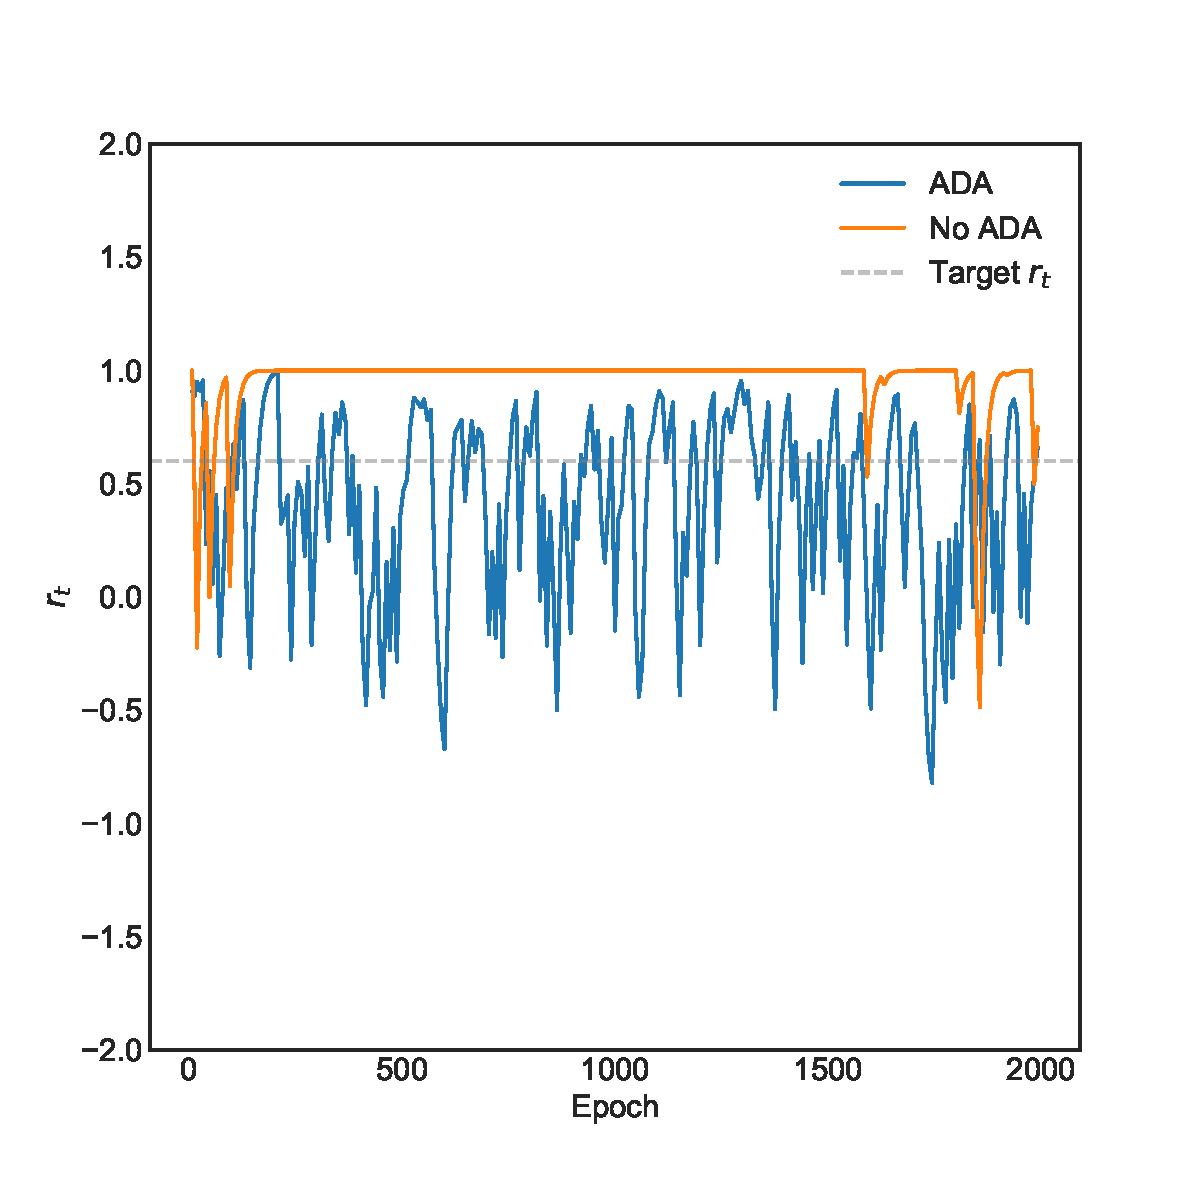
\includegraphics[width=\linewidth]{labels/figs/ada_r_t.pdf}
        \caption{Value of $r_t$ during training.}
        \label{fig:acgan_ada_r_t}
    \end{subfigure} %
    \begin{subfigure}{0.45\textwidth}
        \centering
        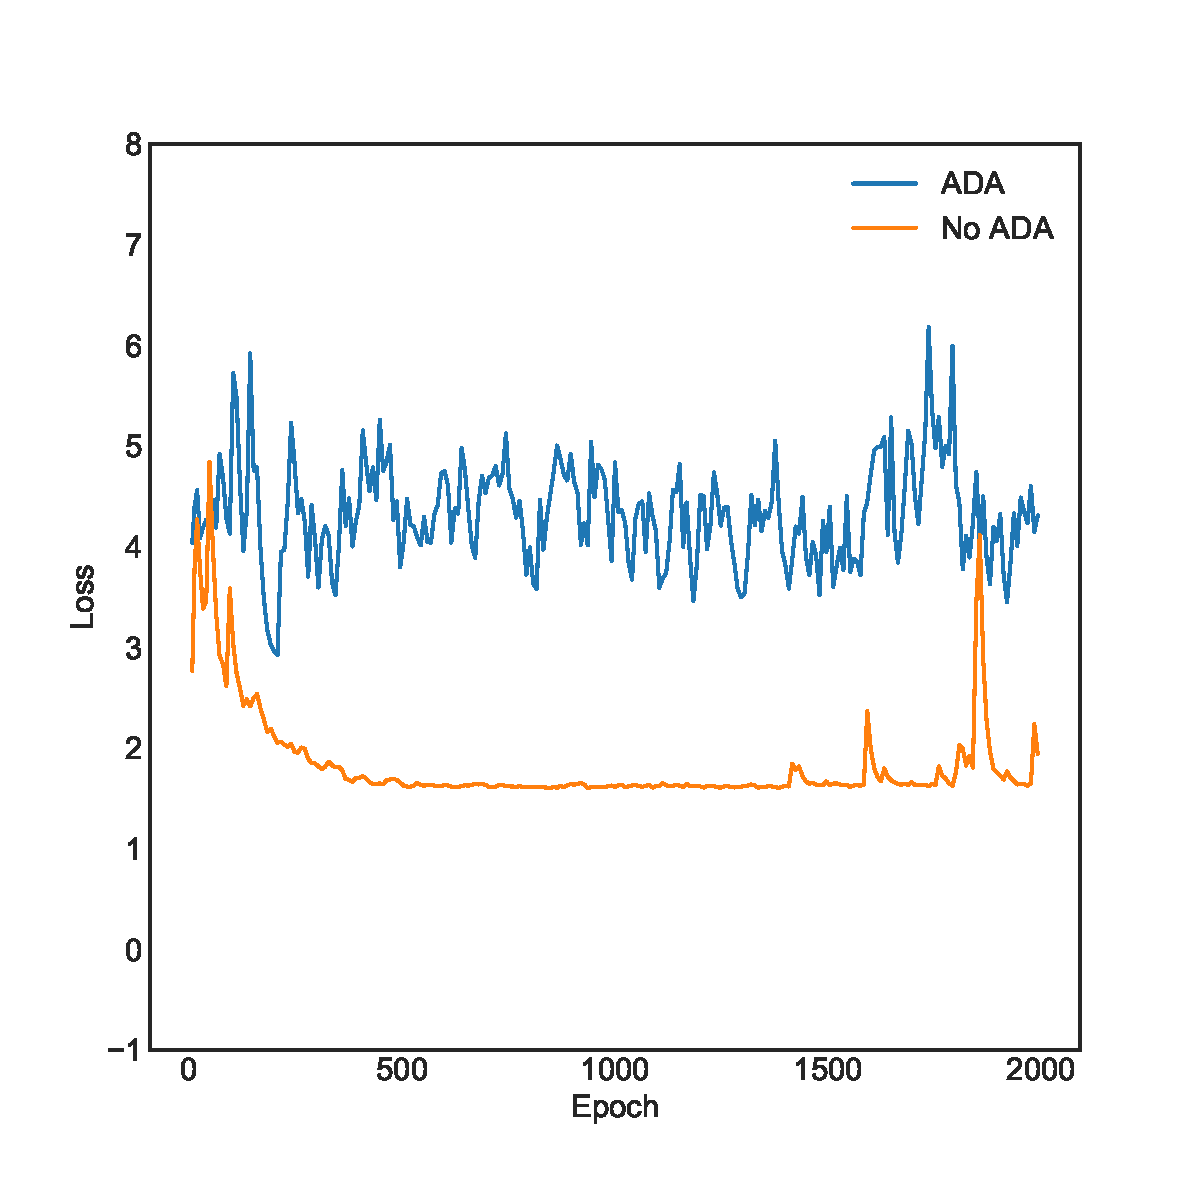
\includegraphics[width=\linewidth]{labels/figs/ada_dis.pdf}
        \caption{Discriminator loss during training.}
        \label{fig:acgan_ada_dis}
    \end{subfigure}
    \caption{Comparison between training with and without ADA.}
    \label{fig:acgan_ada}
\end{figure}

To investigate the importance of ADA to GAN stability, we trained the ACGAN with and without ADA and compared how training developed over time.
From \Cref{fig:acgan_ada}, we can see that without ADA the adversarial discriminator loss quickly collapses.
Note that the total discriminator loss does not go to zero due to the magnitude of the auxiliary losses.
The overfitting heuristic $r_t$ immediately rises to its maximum possible value of 1, and remains there for essentially the rest of training.
The generator is unable to recover from this.
Conversely, when we apply ADA, we are able to use the negative feedback from $r_t$ to increase the probability of augmentations to reduce discriminator overfitting, and thereby keep training relatively stable.

The processing and memory usage required by the ProGAN is significantly higher, which caused batch sizes to be smaller, and overall training times to be much longer.
As a result, we used a batch size of 8 for the ProGAN.
A side-effect of this was that $r_t$ and $p$, which are updated every batch, were much noisier during training for the ProGAN than the ACGAN.

\subsection{Samples}

\begin{figure}[h]
    \centering
    \begin{subfigure}{0.31\textwidth}
        \centering
        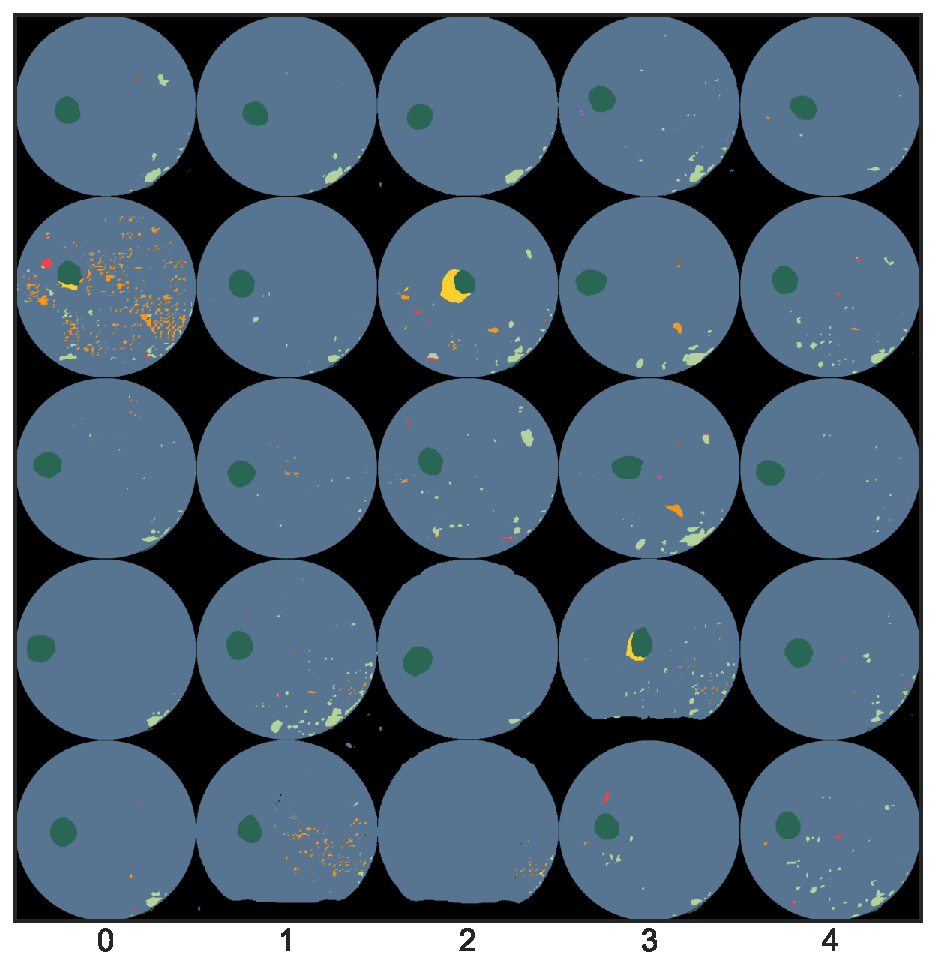
\includegraphics[width=\linewidth]{labels/figs/acgan_sample.pdf}
        \caption{ACGAN}
        \label{fig:acgan_sample}
    \end{subfigure}
    \begin{subfigure}{0.31\textwidth}
        \centering
        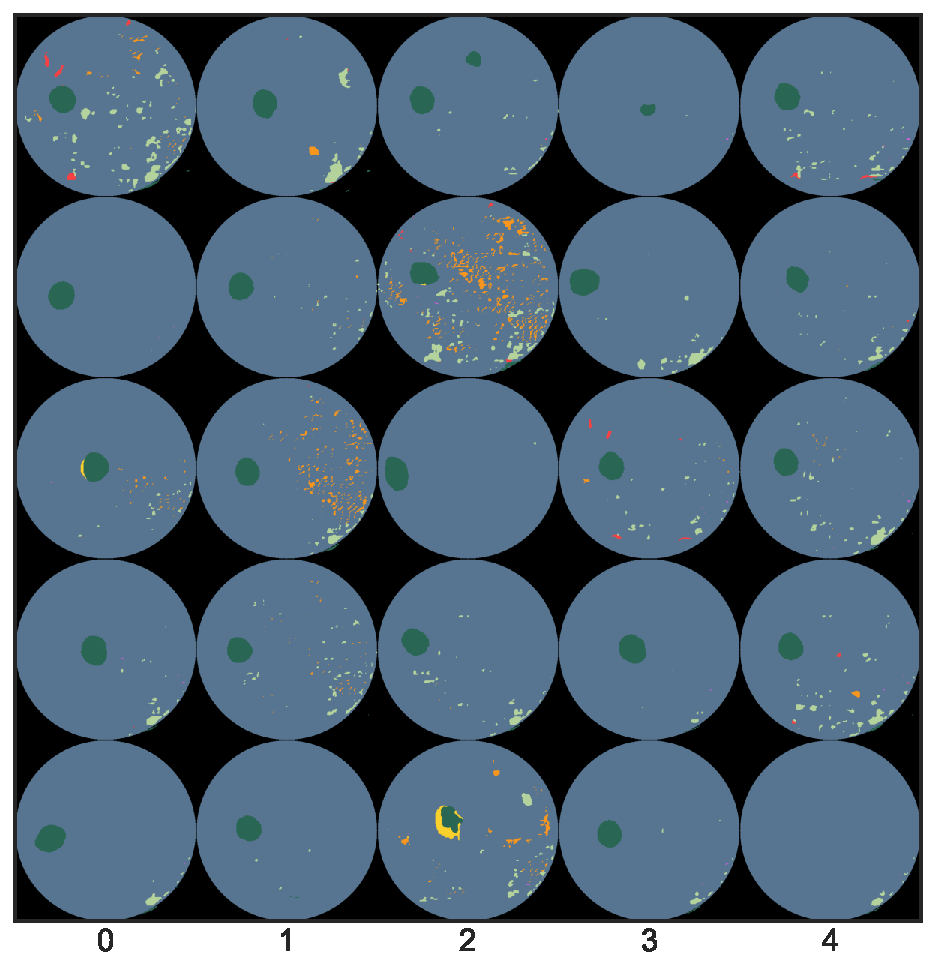
\includegraphics[width=\linewidth]{labels/figs/acgan_mask_sample.pdf}
        \caption{ACGAN + mask}
        \label{fig:acgan_sample_2}
    \end{subfigure}
    \begin{subfigure}{0.31\textwidth}
        \centering
        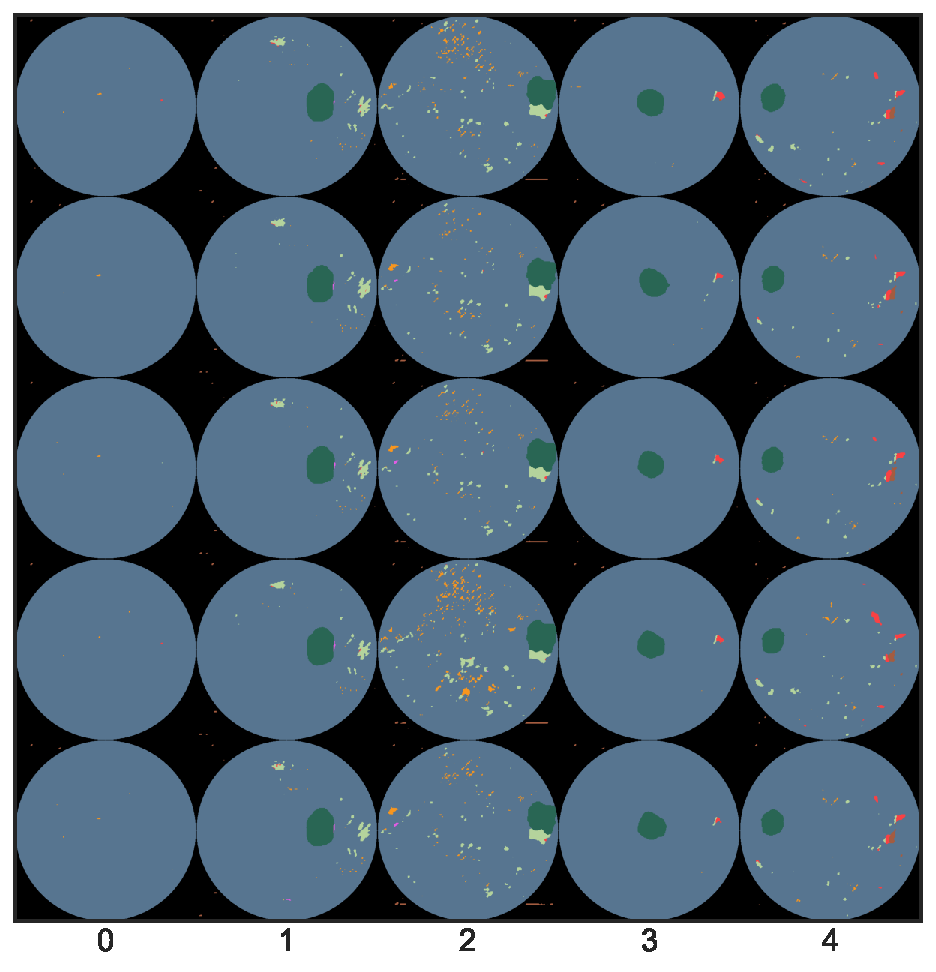
\includegraphics[width=\linewidth]{labels/figs/acgan_concat_sample.pdf}
        \caption{ACGAN + mask, concat.}
        \label{fig:acgan_sample_3}
    \end{subfigure}
    \begin{subfigure}{0.31\textwidth}
        \centering
        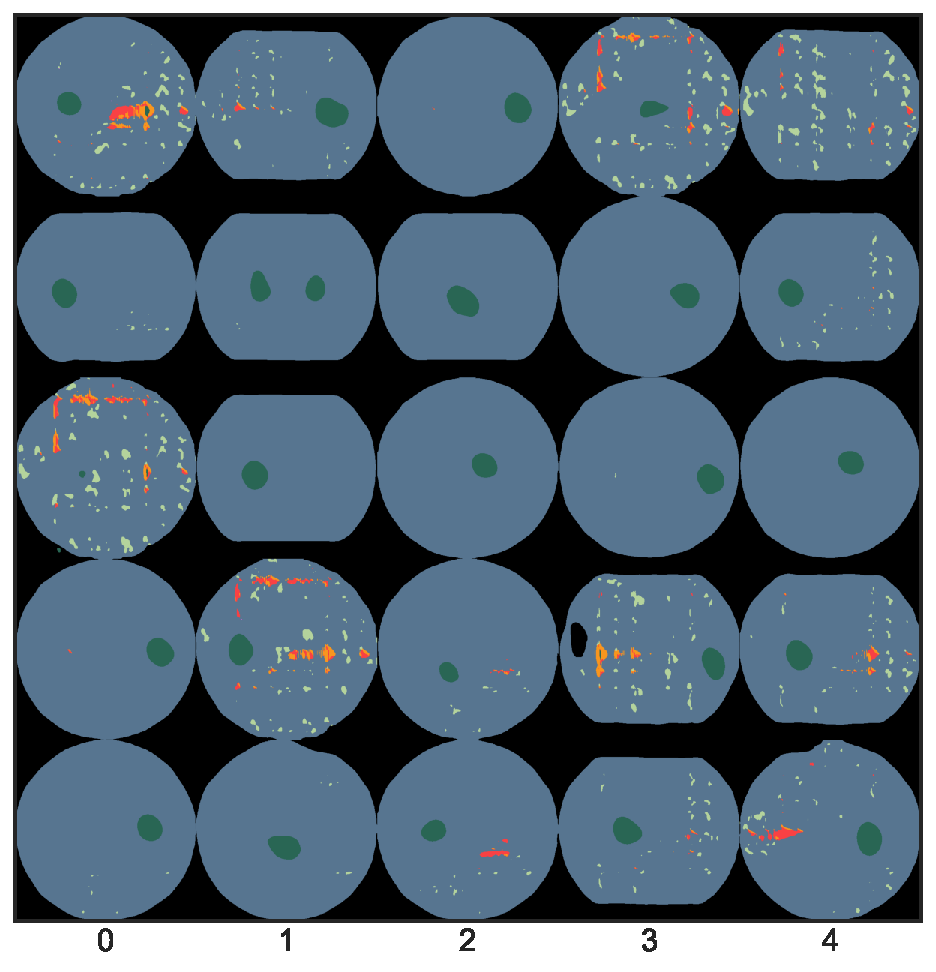
\includegraphics[width=\linewidth]{labels/figs/progan_sample.pdf}
        \caption{ProGAN}
        \label{fig:progan_sample}
    \end{subfigure}
    \begin{subfigure}{0.31\textwidth}
        \centering
        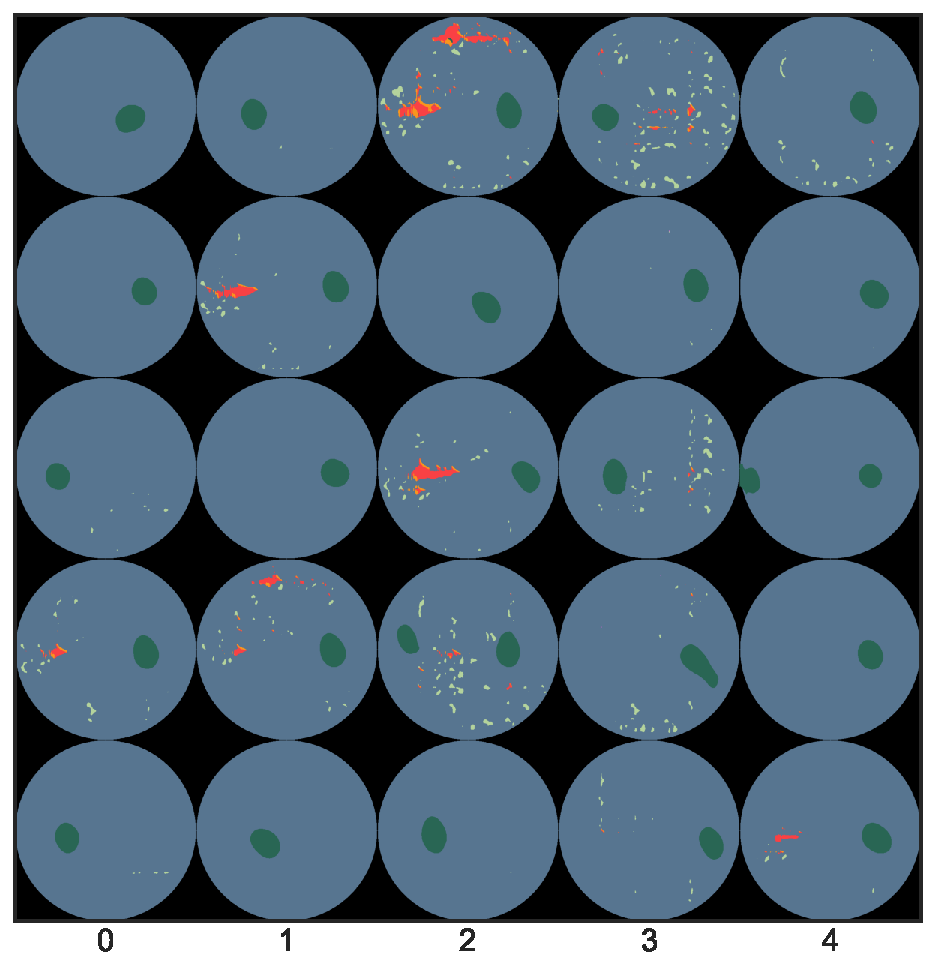
\includegraphics[width=\linewidth]{labels/figs/progan_mask_sample.pdf}
        \caption{ProGAN + mask}
        \label{fig:progan_sample_2}
    \end{subfigure}
    \begin{subfigure}{0.31\textwidth}
        \centering
        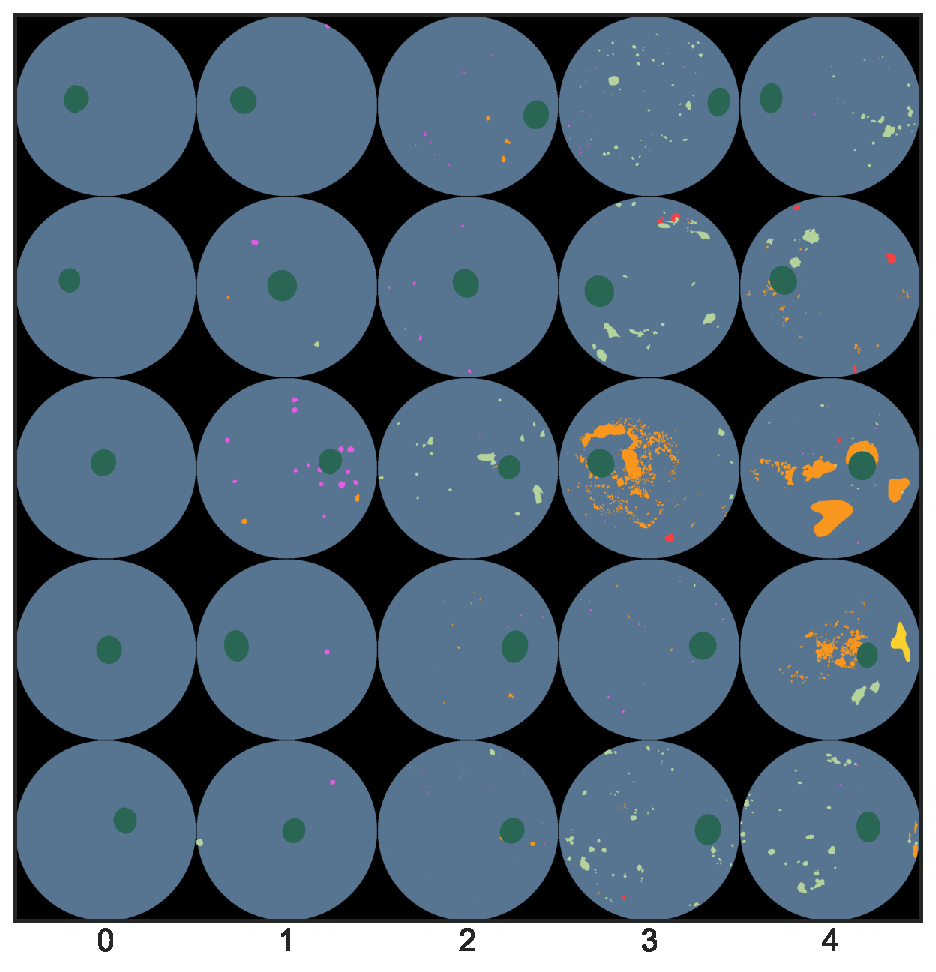
\includegraphics[width=\linewidth]{labels/figs/copypaste_sample.pdf}
        \caption{Copy-Paste}
        \label{fig:copypaste_sample}
    \end{subfigure}
    \caption{Sample of generated semantic labels for each configuration. Columns from left to right correspond to input DR grades 0 through 4.}
    \label{fig:semantic_label_sample}
\end{figure}

A sample of generated images is shown in \Cref{fig:semantic_label_sample}.
From a brief visual examination, the GANs appear have successfully been able to capture the form of the semantic labels.
The conditioning, however, has been less successful.
Only the ACGAN with concatenation has been able to learn a definite conditioning, but it suffers mode collapse within each of the classes.
We can also see a number of recurring modes in the ACGAN and ProGAN samples, which is indicative of low diversity.
Meanwhile, the copy-pasted data shows a diverse range of samples, and is clearly well-conditioned. 
Despite this, there are some instances where the optic disc has been pasted directly on top lesions, which is unrealistic.
The ``mask'' variants have an additional post-processing step applied in which the fundus boundary is masked as a circle.
This is in response to a failure mode discussed in the next section.

\subsection{Common Failure Modes}

\begin{figure}[h]
    \centering
    \begin{subfigure}[t]{0.19\textwidth}
        \centering
        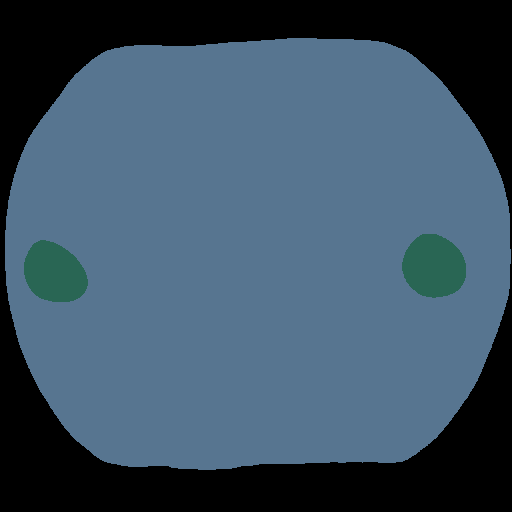
\includegraphics[width=\linewidth]{labels/figs/two-od.png}
        \caption{Multiple optic discs.}
        \label{fig:two_od}
    \end{subfigure} %
    \hfill
    \begin{subfigure}[t]{0.19\textwidth}
        \centering
        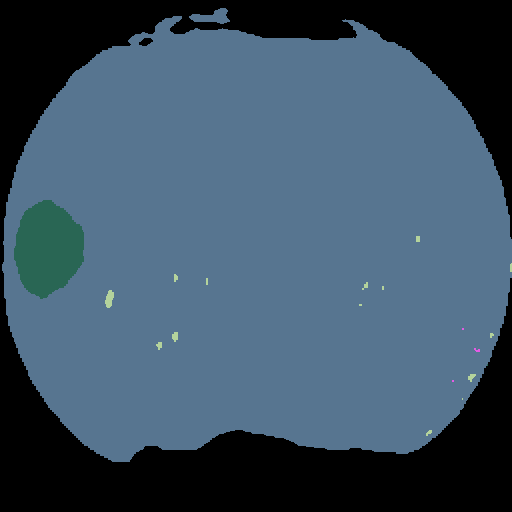
\includegraphics[width=\linewidth]{labels/figs/malformed-fundus.png}
        \caption{Malformed fundus.}
        \label{fig:malformed_fundus}
    \end{subfigure} %
    \hfill
    \begin{subfigure}[t]{0.19\textwidth}
        \centering
        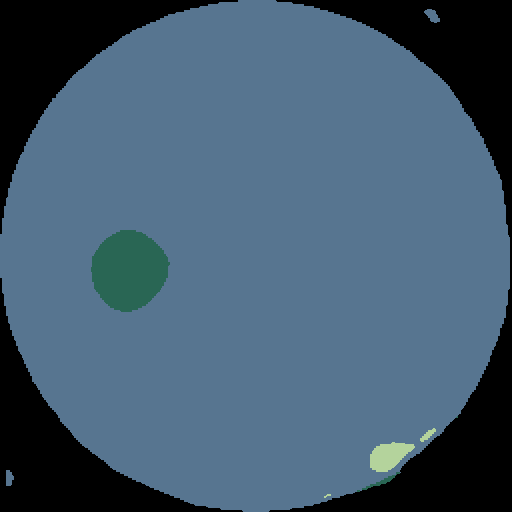
\includegraphics[width=\linewidth]{labels/figs/spurious-pixels.png}
        \caption{Spurious pixels.}
        \label{fig:spurious_pixels}
    \end{subfigure} %
    \hfill
    \begin{subfigure}[t]{0.19\textwidth}
        \centering
        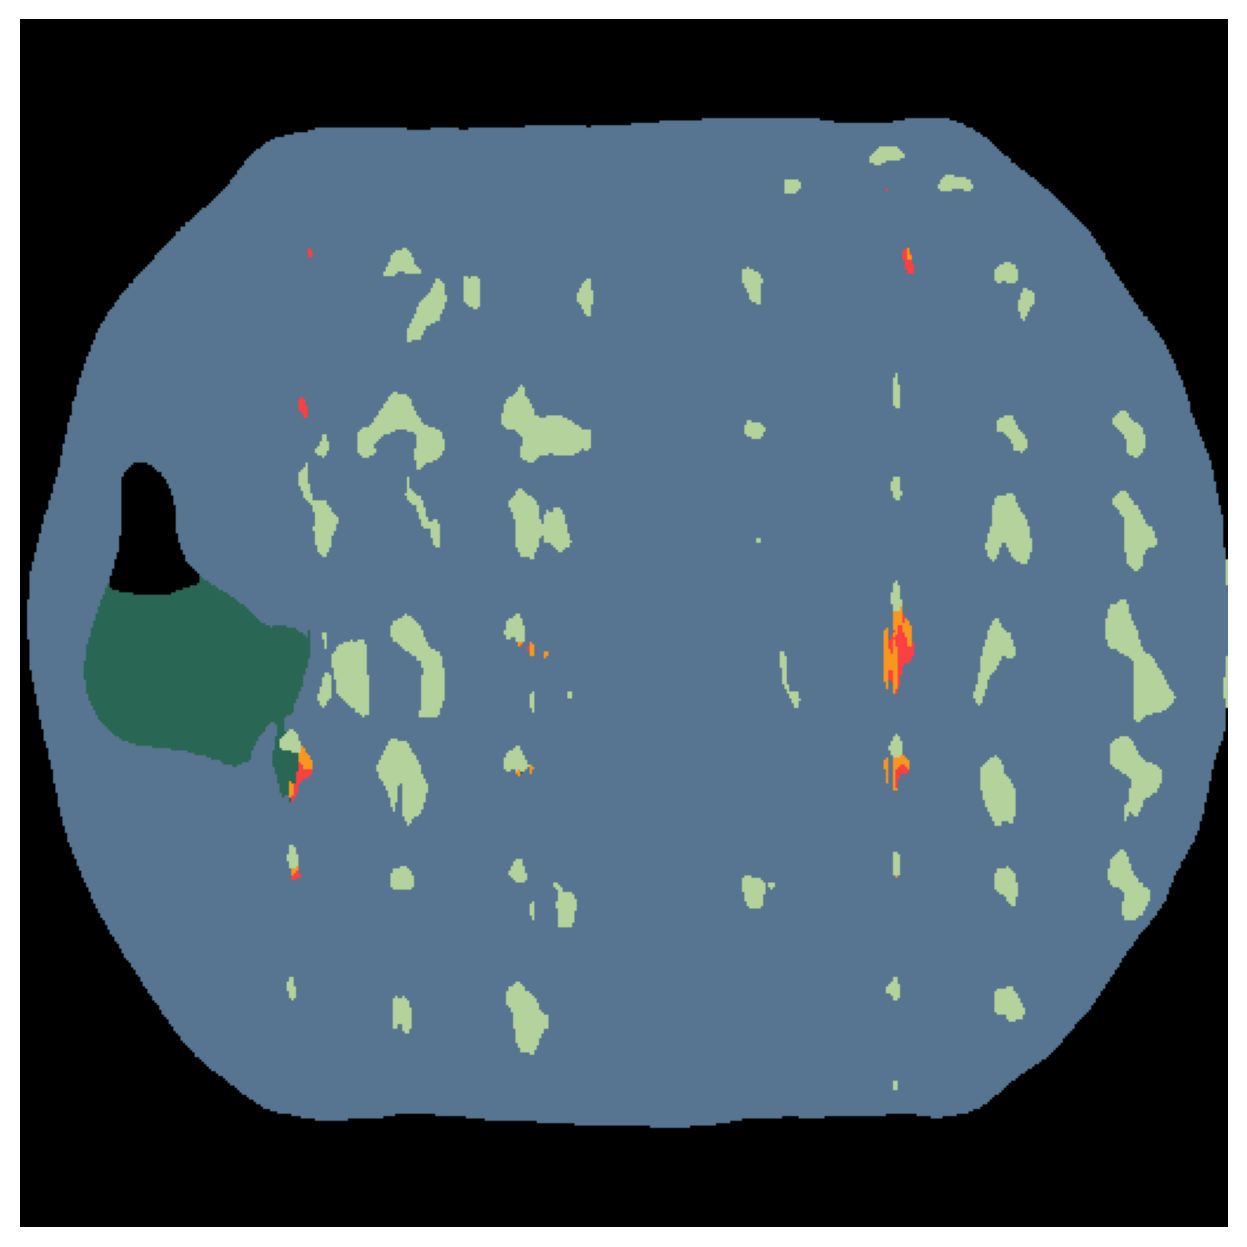
\includegraphics[width=\linewidth]{labels/figs/hole.png}
        \caption{Holes.}
        \label{fig:holes}
    \end{subfigure} %
    \hfill
    \begin{subfigure}[t]{0.19\textwidth}
        \centering
        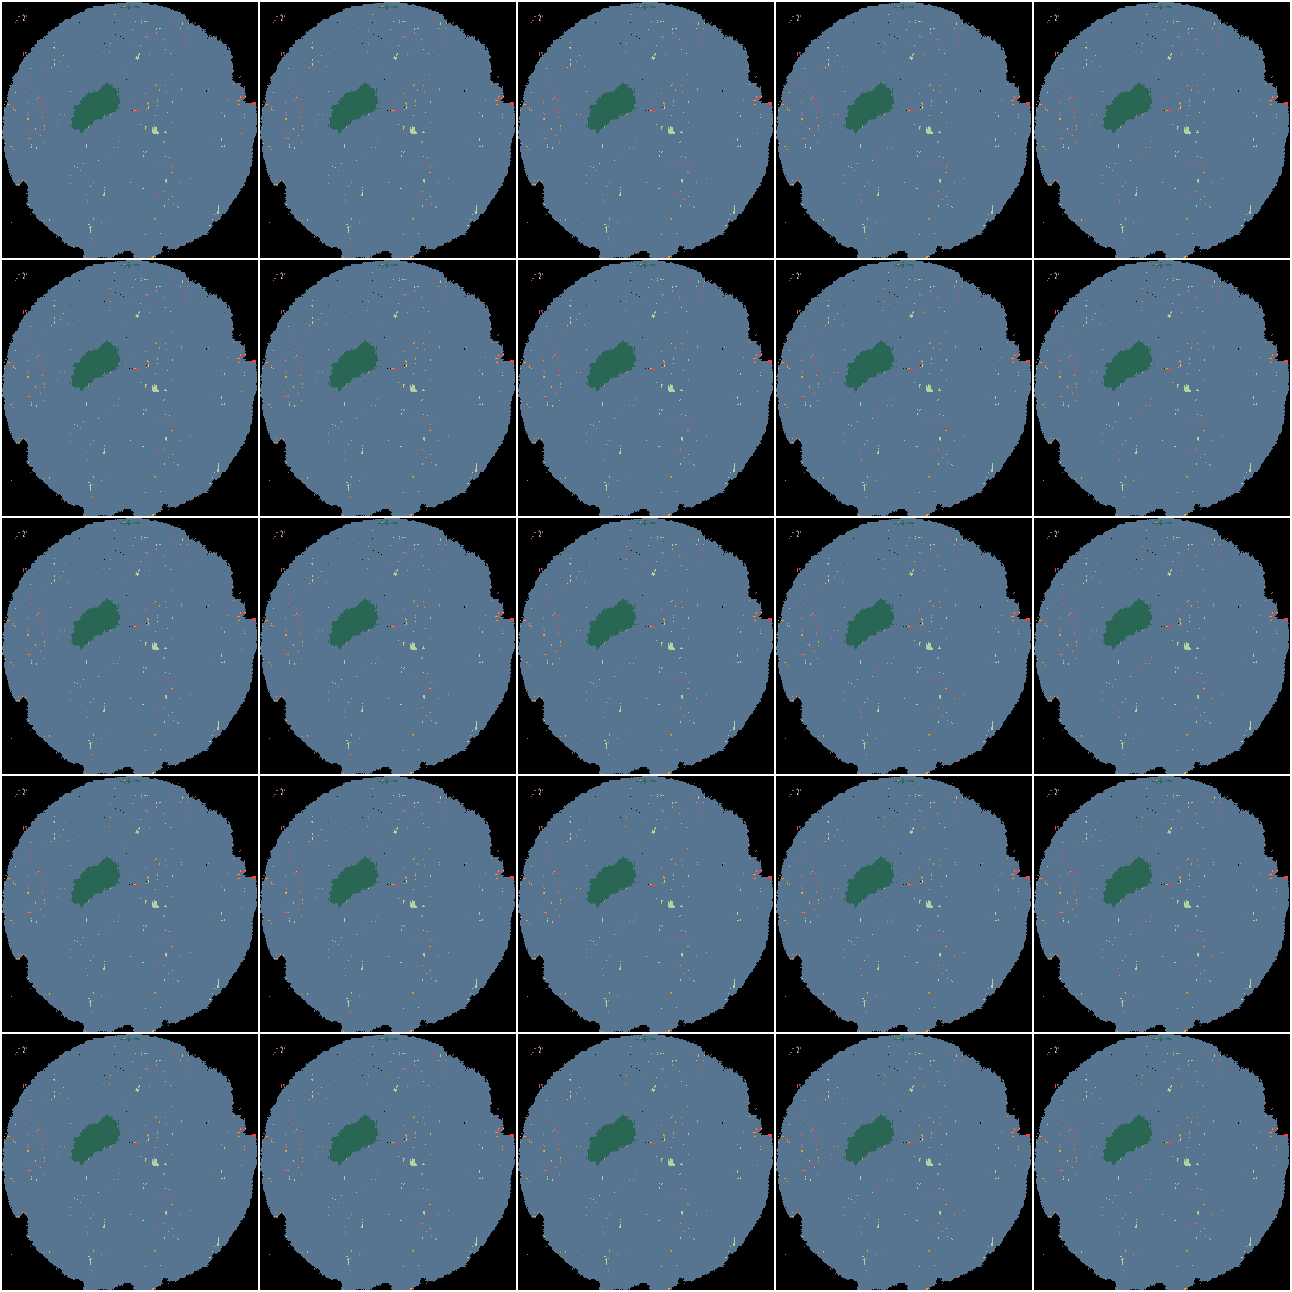
\includegraphics[width=\linewidth]{labels/figs/mode-collapse.png}
        \caption{Mode collapse.}
        \label{fig:mode_collapse}
    \end{subfigure} %
    \caption{Examples of common failure modes.}
    \label{fig:acgan_bad_sample}
\end{figure}

The models still display a number of failure modes which are yet to be addressed in the current iteration of this work.

\begin{description}
    \item[Multiple Optic Discs] \hfill \\ 
    There is a tendency to generate multiple optic discs, which is not possible in the source data. 
    Example shown in \Cref{fig:two_od}.
    
    \item[Malformed Fundus] \hfill \\ 
    Both GAN types encountered difficulty with generating geometric shapes, such as the circular fundus mask.
    One mitigation is to remove this responsibility from the generator and simply mask out the fundus as a post-processing step.
    Example shown in \Cref{fig:malformed_fundus}.
    
    \item[Spurious Pixels] \hfill \\ 
    If the GAN is over-trained, there is a point at which spurious pixels outside of the fundus boundary are generated.
    These kinds of artefacts are obviously unrealistic and not desirable.
    Example shown in \Cref{fig:spurious_pixels}.
    
    \item[Holes] \hfill \\ 
    Some images exhibit ``tears'' or gaps in the semantic labels. This is particularly prevalent with the ProGAN. 
    Example shown in \Cref{fig:holes}.
    
    \item[Low Diversity/Mode Collapse] \hfill \\ 
    As mentioned, the GANs can exhibit low diversity, even if this does not quite extend to total mode collapse.
    For instance, one can see from the ACGAN samples that the optic disc is generated in approximately the same spot in almost all samples.
    Without diversity, downstream models will be prone to overfitting to the synthetic data, decreasing performance. 
    This happens when the discriminator is too strong, which implies that we may need to inhibit the discriminator even further.
    Example shown in \Cref{fig:mode_collapse}.
\end{description}

\subsection{Results}

\begin{table}[h]
    \centering
    \begin{tabular}{lrrrrrr}
    \toprule
        Configuration & FID$\downarrow$ & Accuracy$\uparrow$ & Precision$\uparrow$ & Recall$\uparrow$ & $F_1$$\uparrow$ & $\kappa$$\uparrow$ \\
    \midrule
        Validation & 17.118 & 0.709 & 0.700 & 0.741 & 0.710 & 0.739 \\
    \midrule
        ACGAN & 64.388 & 0.191 & 0.249 & 0.187 & 0.115 & -0.004 \\
        + mask & 44.674 & 0.195 & 0.194 & 0.195 & 0.154 & 0.001 \\
        + mask, concatenation & 80.743 & 0.037 & 0.216 & 0.036 & 0.027 & 0.051 \\
    \midrule
        ProGAN & 51.970 & 0.206 & 0.194 & 0.205 & 0.142 & 0.020 \\
        + mask & 46.044 & 0.200 & 0.189 & 0.199 & 0.176 & 0.018 \\
    \midrule
        Copy-Paste & \textbf{21.717} & \textbf{0.691} & \textbf{0.688} & \textbf{0.691} & \textbf{0.686} & \textbf{0.807} \\
    \bottomrule
    \end{tabular}
    \caption{Metrics assessing the image and conditioning quality for each generation method. Best results for each metric in bold (excluding the baseline).}
    \label{tab:acgan_results}
\end{table}

To evaluate image quality, we compute the FID score between the coloured semantic labels of the training set and those of the target dataset.
Even though the FID is designed for natural looking images (after all, the Inception network is trained on Image-Net), and the semantic image colours are chosen arbitrarily, it seems to function as a fairly good proxy for visual quality and diversity regardless.
To evaluate the strength of DR grade conditioning, we trained a ResNet-50 network for 100 epochs on the 9-channel semantic labels of the FGADR subset of the real training data (since only these have annotations for DR severity labels).
We use this network to perform inference on generated data, and retrieve the accuracy, precision, recall, $F_1$, and $\kappa$ achieved.
This model was trained on one Nvidia GeForce GTX 1080 for 100 epochs over 2 hours.

Quantitative results of these experiments are reported in \Cref{tab:acgan_results}.
In addition to metrics on the synthetic datasets, we also include metrics on the real validation dataset as a baseline.
The ``mask'' configurations refer to using a circle mask for the retinal fundus boundary, and the ``concatenation'' configuration refers to concatenating the class vector instead of taking the Hadamard product.

From these, we find that copy-paste generated samples yield the best metrics across the board, by quite some margin -- even yielding a greater $\kappa$ than the validation set.
Moreover, our fears about poor conditioning are confirmed, with each GAN-based method displaying classifying power which is effectively no better than random in their samples.
The variants with masked retinal fundus boundaries exhibited a marked improvement in FID, which indicates that this is a simple, but promising, post-processing technique.

Of the GANs, the ACGAN with concatenation had the largest $\kappa$ (while still being low compared to real data).
However, it had a much higher FID, despite the individual generated images appearing similar to the others.
This is because the FID score attempts to capture diversity as well as image quality, and these samples exhibit very little diversity owing to mode collapse during training.

In addition to the quality of images, training and inference time are also important factors for practicality.
In \Cref{tab:time} we report the mean training time of each model, as well as the average inference time for 1000 images.

\begin{table}[h]
    \centering
    \begin{tabular}{lrrr}
        \toprule
        Configuration & Time Per Epoch (s) $\downarrow$ & \multicolumn{2}{r}{Inference Time$\downarrow$ (s)} \\
        \midrule
        ACGAN & 36.9 & \textbf{13.08} & $\pm$ 0.933 \\
        \midrule
        ProGAN & 112.5 & 35.51 & $\pm$ 0.100 \\
        \midrule
        Copy-Paste & \textbf{--} & 183.29 & $\pm$ 1.304 \\
        \bottomrule
    \end{tabular}
    \caption{Training and inference time for different semantic label generation methods. We report the mean of three runs and the standard error of the mean. Best results for each metric in bold.}
    \label{tab:time}
\end{table}

These experiments were run on a machine with a Nvidia GeForce GTX 1080 Ti GPU, Intel i7-7700K 4.20GHz CPU, and 32 GB of memory.
For inference, we use a batch size of 128 for the ACGAN and 8 for the ProGAN.
The ``time per epoch'' figure for the ProGAN is given as an average across the entire duration of training, despite smaller resolutions taking significantly less time than higher resolutions.

Being able to generate images at twice the resolution, and as a much larger network overall, the ProGAN is over 3 times slower to train than the ACGAN.
It also incurs a similar performance penalty during inference.
This can be partly attributed to the fact that batch size is far more limited for the ProGAN.
Meanwhile, data generation via copy-pasting does not require any form of training. 
While copy-paste appears performs poorly here in terms of inference time, it is worth bearing in mind that this implementation is far from optimised.
For instance, no GPU acceleration is performed, nor is it multi-threaded.
This leaves large room for improvement, and could feasibly be faster than the neural networks when properly optimised.
